\documentclass[11pt]{article}
\usepackage[review]{acl}
\usepackage{times}
\usepackage{latexsym}
\usepackage[T1]{fontenc}
\usepackage[utf8]{inputenc}
\usepackage{microtype}
\usepackage{inconsolata}
\usepackage{graphicx}
\usepackage{booktabs}
\usepackage{amsmath}
\usepackage{xspace}
\usepackage[most]{tcolorbox}
% lineno 5.7 with LaTeX 2025+ records the column one column late, so review-mode line numbers land on the wrong
% side; restore lineno's older column tracking.
\makeatletter
\IfPackageLoadedT{lineno}{%
  \RemoveFromHook{build/column/before}[lineno]%
  \AtBeginDocument{\def\@LN@makecol{\@LN@orig@makecol
    \setbox\@outputbox\vbox{\boxmaxdepth\@maxdepth
      \protected@write\@auxout{}{\string\def\string\@LN@column{\if@firstcolumn1\else2\fi}}%
      \box\@outputbox}}}}
\makeatother
% generated by paper_tables.py
\newcommand{\R}[1]{\ifcsname r@#1\endcsname\csname r@#1\endcsname\else\textbf{??}\fi}
\expandafter\def\csname r@adir.cross.cos.hi\endcsname{0.48}
\expandafter\def\csname r@adir.cross.cos.lo\endcsname{0.03}
\expandafter\def\csname r@adir.cross.m2t.hi\endcsname{64}
\expandafter\def\csname r@adir.cross.m2t.lo\endcsname{49}
\expandafter\def\csname r@adir.cross.n\endcsname{5}
\expandafter\def\csname r@adir.cross.t2m.hi\endcsname{79}
\expandafter\def\csname r@adir.cross.t2m.lo\endcsname{53}
\expandafter\def\csname r@adir.math.abscos.hi\endcsname{0.76}
\expandafter\def\csname r@adir.math.auth.hi\endcsname{84}
\expandafter\def\csname r@adir.math.auth.lo\endcsname{66}
\expandafter\def\csname r@adir.math.cos.hi\endcsname{+0.76}
\expandafter\def\csname r@adir.math.cos.lo\endcsname{+0.43}
\expandafter\def\csname r@adir.math.cosaa.hi\endcsname{+0.36}
\expandafter\def\csname r@adir.math.cosaa.lo\endcsname{$-$0.15}
\expandafter\def\csname r@adir.math.dir.all\endcsname{65.3}
\expandafter\def\csname r@adir.math.dir.diff\endcsname{67.4}
\expandafter\def\csname r@adir.math.dir.same\endcsname{59.6}
\expandafter\def\csname r@adir.math.n\endcsname{7}
\expandafter\def\csname r@adir.math.perp.all\endcsname{64.2}
\expandafter\def\csname r@adir.math.perp.diff\endcsname{65.2}
\expandafter\def\csname r@adir.math.perp.same\endcsname{61.5}
\expandafter\def\csname r@adir.math.removed.half\endcsname{1}
\expandafter\def\csname r@adir.math.removed.hi\endcsname{103}
\expandafter\def\csname r@adir.math.removed.lo\endcsname{-53}
\expandafter\def\csname r@adir.math.removed.mean\endcsname{8}
\expandafter\def\csname r@adir.math.verdict.all\endcsname{57.5}
\expandafter\def\csname r@adir.math.verdict.diff\endcsname{56.8}
\expandafter\def\csname r@adir.math.verdict.same\endcsname{59.3}
\expandafter\def\csname r@adir.math.xfer.hi\endcsname{91}
\expandafter\def\csname r@adir.math.xfer.lo\endcsname{35}
\expandafter\def\csname r@adir.mmlu.abscos.hi\endcsname{0.19}
\expandafter\def\csname r@adir.mmlu.auth.hi\endcsname{85}
\expandafter\def\csname r@adir.mmlu.auth.lo\endcsname{78}
\expandafter\def\csname r@adir.mmlu.cos.hi\endcsname{+0.19}
\expandafter\def\csname r@adir.mmlu.cos.lo\endcsname{$-$0.05}
\expandafter\def\csname r@adir.mmlu.cosaa.hi\endcsname{$-$0.47}
\expandafter\def\csname r@adir.mmlu.cosaa.lo\endcsname{$-$0.58}
\expandafter\def\csname r@adir.mmlu.dir.all\endcsname{61.8}
\expandafter\def\csname r@adir.mmlu.dir.diff\endcsname{63.7}
\expandafter\def\csname r@adir.mmlu.dir.same\endcsname{55.6}
\expandafter\def\csname r@adir.mmlu.n\endcsname{6}
\expandafter\def\csname r@adir.mmlu.perp.all\endcsname{56.3}
\expandafter\def\csname r@adir.mmlu.perp.diff\endcsname{56.5}
\expandafter\def\csname r@adir.mmlu.perp.same\endcsname{55.4}
\expandafter\def\csname r@adir.mmlu.removed.half\endcsname{4}
\expandafter\def\csname r@adir.mmlu.removed.hi\endcsname{85}
\expandafter\def\csname r@adir.mmlu.removed.lo\endcsname{42}
\expandafter\def\csname r@adir.mmlu.removed.mean\endcsname{61}
\expandafter\def\csname r@adir.mmlu.verdict.all\endcsname{52.4}
\expandafter\def\csname r@adir.mmlu.verdict.diff\endcsname{52.0}
\expandafter\def\csname r@adir.mmlu.verdict.same\endcsname{53.6}
\expandafter\def\csname r@adir.mmlu.xfer.hi\endcsname{33}
\expandafter\def\csname r@adir.mmlu.xfer.lo\endcsname{27}
\expandafter\def\csname r@auth.diff\endcsname{+11.6}
\expandafter\def\csname r@auth.diff.ci\endcsname{+11.6 [+10.8, +12.5]}
\expandafter\def\csname r@auth.diff.direct\endcsname{64.2}
\expandafter\def\csname r@auth.diff.hi\endcsname{+17.7}
\expandafter\def\csname r@auth.diff.k\endcsname{19}
\expandafter\def\csname r@auth.diff.lo\endcsname{+6.2}
\expandafter\def\csname r@auth.diff.sig\endcsname{19}
\expandafter\def\csname r@auth.diff.verdict\endcsname{52.7}
\expandafter\def\csname r@auth.diffm.ci\endcsname{+12.1 [+11.2, +13.0]}
\expandafter\def\csname r@auth.diffm.k\endcsname{12}
\expandafter\def\csname r@auth.dir.hi\endcsname{85}
\expandafter\def\csname r@auth.dir.lo\endcsname{66}
\expandafter\def\csname r@auth.dir.med\endcsname{80}
\expandafter\def\csname r@auth.same\endcsname{+1.9}
\expandafter\def\csname r@auth.same.ci\endcsname{+1.9 [+0.5, +3.2]}
\expandafter\def\csname r@auth.same.direct\endcsname{57.8}
\expandafter\def\csname r@auth.same.hi\endcsname{+7.5}
\expandafter\def\csname r@auth.same.k\endcsname{12}
\expandafter\def\csname r@auth.same.lo\endcsname{$-$2.9}
\expandafter\def\csname r@auth.same.sig\endcsname{2}
\expandafter\def\csname r@auth.same.verdict\endcsname{55.8}
\expandafter\def\csname r@auth.ver.hi\endcsname{86}
\expandafter\def\csname r@auth.ver.lo\endcsname{75}
\expandafter\def\csname r@big.bbeh.auth.dir\endcsname{100}
\expandafter\def\csname r@big.bbeh.auth.ver\endcsname{100}
\expandafter\def\csname r@big.bbeh.gap\endcsname{+4.6}
\expandafter\def\csname r@big.bbeh.gap0\endcsname{+6.0}
\expandafter\def\csname r@big.bbeh.knows\endcsname{63.2}
\expandafter\def\csname r@big.bbeh.pool.cot.rank.ci\endcsname{$-$0.7 [$-$5.4, +4.2]}
\expandafter\def\csname r@big.bbeh.pool.cot_sum.rank.ci\endcsname{+3.9 [$-$1.1, +8.6]}
\expandafter\def\csname r@big.bbeh.pool.direct.rank.ci\endcsname{+6.0 [+1.2, +11.0]}
\expandafter\def\csname r@big.bbeh.pool.sum.rank.ci\endcsname{+4.5 [+1.6, +7.4]}
\expandafter\def\csname r@big.bbeh.pool.x11.rank.ci\endcsname{+1.4 [$-$1.2, +4.0]}
\expandafter\def\csname r@big.bbeh.pool.x4.rank.ci\endcsname{+1.0 [$-$0.4, +2.5]}
\expandafter\def\csname r@big.bbeh.says\endcsname{58.6}
\expandafter\def\csname r@big.bbeh.sm.qwen.cot.rank.abs\endcsname{58.0}
\expandafter\def\csname r@big.bbeh.sm.qwen.cot.rank.ci\endcsname{+2.8 [$-$0.1, +5.4]}
\expandafter\def\csname r@big.bbeh.sm.qwen.cot_sum.rank.abs\endcsname{56.6}
\expandafter\def\csname r@big.bbeh.sm.qwen.cot_sum.rank.ci\endcsname{+1.4 [$-$1.6, +4.4]}
\expandafter\def\csname r@big.bbeh.sm.qwen.direct.rank.abs\endcsname{56.1}
\expandafter\def\csname r@big.bbeh.sm.qwen.direct.rank.ci\endcsname{+0.9 [$-$2.4, +4.2]}
\expandafter\def\csname r@big.bbeh.sm.qwen.nq\endcsname{311}
\expandafter\def\csname r@big.bbeh.sm.qwen.sum.rank.abs\endcsname{57.8}
\expandafter\def\csname r@big.bbeh.sm.qwen.sum.rank.ci\endcsname{+2.6 [+0.4, +4.9]}
\expandafter\def\csname r@big.bbeh.sm.qwen.verdict.rank\endcsname{55.2}
\expandafter\def\csname r@big.bbeh.sm.qwen.x11.rank.abs\endcsname{54.7}
\expandafter\def\csname r@big.bbeh.sm.qwen.x11.rank.ci\endcsname{$-$0.5 [$-$2.6, +1.6]}
\expandafter\def\csname r@big.bbeh.sm.qwen.x4.rank.abs\endcsname{56.1}
\expandafter\def\csname r@big.bbeh.sm.qwen.x4.rank.ci\endcsname{+0.9 [+0.0, +1.9]}
\expandafter\def\csname r@big.bbeh.solved\endcsname{15}
\expandafter\def\csname r@big.math.auth.dir\endcsname{72}
\expandafter\def\csname r@big.math.auth.ver\endcsname{76}
\expandafter\def\csname r@big.math.gap\endcsname{+4.5}
\expandafter\def\csname r@big.math.gap0\endcsname{+4.4}
\expandafter\def\csname r@big.math.knows\endcsname{66.3}
\expandafter\def\csname r@big.math.pool.cot.rank.ci\endcsname{+0.7 [$-$1.5, +2.9]}
\expandafter\def\csname r@big.math.pool.cot_sum.rank.ci\endcsname{+3.8 [+1.9, +5.8]}
\expandafter\def\csname r@big.math.pool.direct.rank.ci\endcsname{+4.4 [+2.3, +6.5]}
\expandafter\def\csname r@big.math.pool.sum.rank.ci\endcsname{+2.6 [+1.2, +3.9]}
\expandafter\def\csname r@big.math.pool.x11.rank.ci\endcsname{+0.5 [$-$1.2, +2.1]}
\expandafter\def\csname r@big.math.pool.x4.rank.ci\endcsname{+1.7 [+0.5, +2.9]}
\expandafter\def\csname r@big.math.says\endcsname{61.9}
\expandafter\def\csname r@big.math.sm.olmo.cot.rank.abs\endcsname{62.8}
\expandafter\def\csname r@big.math.sm.olmo.cot.rank.ci\endcsname{+0.2 [$-$5.0, +5.8]}
\expandafter\def\csname r@big.math.sm.olmo.cot_sum.rank.abs\endcsname{63.1}
\expandafter\def\csname r@big.math.sm.olmo.cot_sum.rank.ci\endcsname{+0.5 [$-$3.3, +4.1]}
\expandafter\def\csname r@big.math.sm.olmo.direct.rank.abs\endcsname{64.4}
\expandafter\def\csname r@big.math.sm.olmo.direct.rank.ci\endcsname{+1.8 [$-$1.7, +4.9]}
\expandafter\def\csname r@big.math.sm.olmo.nq\endcsname{89}
\expandafter\def\csname r@big.math.sm.olmo.sum.rank.abs\endcsname{63.3}
\expandafter\def\csname r@big.math.sm.olmo.sum.rank.ci\endcsname{+0.7 [$-$1.2, +2.4]}
\expandafter\def\csname r@big.math.sm.olmo.verdict.rank\endcsname{62.6}
\expandafter\def\csname r@big.math.sm.olmo.x11.rank.abs\endcsname{58.9}
\expandafter\def\csname r@big.math.sm.olmo.x11.rank.ci\endcsname{$-$3.7 [$-$7.8, $-$0.1]}
\expandafter\def\csname r@big.math.sm.olmo.x4.rank.abs\endcsname{62.6}
\expandafter\def\csname r@big.math.sm.olmo.x4.rank.ci\endcsname{+0.0 [$-$2.0, +1.8]}
\expandafter\def\csname r@big.math.sm.qwen.cot.rank.abs\endcsname{63.3}
\expandafter\def\csname r@big.math.sm.qwen.cot.rank.ci\endcsname{+0.4 [$-$1.8, +2.6]}
\expandafter\def\csname r@big.math.sm.qwen.cot_sum.rank.abs\endcsname{63.8}
\expandafter\def\csname r@big.math.sm.qwen.cot_sum.rank.ci\endcsname{+0.8 [$-$1.3, +2.8]}
\expandafter\def\csname r@big.math.sm.qwen.direct.rank.abs\endcsname{64.0}
\expandafter\def\csname r@big.math.sm.qwen.direct.rank.ci\endcsname{+1.1 [$-$1.4, +3.3]}
\expandafter\def\csname r@big.math.sm.qwen.nq\endcsname{280}
\expandafter\def\csname r@big.math.sm.qwen.sum.rank.abs\endcsname{64.6}
\expandafter\def\csname r@big.math.sm.qwen.sum.rank.ci\endcsname{+1.7 [+0.3, +3.0]}
\expandafter\def\csname r@big.math.sm.qwen.verdict.rank\endcsname{62.9}
\expandafter\def\csname r@big.math.sm.qwen.x11.rank.abs\endcsname{63.1}
\expandafter\def\csname r@big.math.sm.qwen.x11.rank.ci\endcsname{+0.1 [$-$1.9, +1.9]}
\expandafter\def\csname r@big.math.sm.qwen.x4.rank.abs\endcsname{63.7}
\expandafter\def\csname r@big.math.sm.qwen.x4.rank.ci\endcsname{+0.8 [$-$0.7, +2.1]}
\expandafter\def\csname r@big.math.solved\endcsname{30}
\expandafter\def\csname r@big.mmlu.auth.dir\endcsname{67}
\expandafter\def\csname r@big.mmlu.auth.ver\endcsname{72}
\expandafter\def\csname r@big.mmlu.gap\endcsname{+1.4}
\expandafter\def\csname r@big.mmlu.gap0\endcsname{+1.7}
\expandafter\def\csname r@big.mmlu.knows\endcsname{66.4}
\expandafter\def\csname r@big.mmlu.pool.cot.rank.ci\endcsname{$-$2.4 [$-$4.0, $-$0.8]}
\expandafter\def\csname r@big.mmlu.pool.cot_sum.rank.ci\endcsname{+1.0 [$-$0.2, +2.1]}
\expandafter\def\csname r@big.mmlu.pool.direct.rank.ci\endcsname{+1.7 [+0.5, +3.0]}
\expandafter\def\csname r@big.mmlu.pool.sum.rank.ci\endcsname{+0.7 [$-$0.1, +1.5]}
\expandafter\def\csname r@big.mmlu.pool.x11.rank.ci\endcsname{$-$0.2 [$-$1.2, +1.0]}
\expandafter\def\csname r@big.mmlu.pool.x4.rank.ci\endcsname{+0.5 [$-$0.3, +1.3]}
\expandafter\def\csname r@big.mmlu.says\endcsname{65.0}
\expandafter\def\csname r@big.mmlu.sm.olmo.cot.rank.abs\endcsname{46.2}
\expandafter\def\csname r@big.mmlu.sm.olmo.cot.rank.ci\endcsname{$-$4.4 [$-$9.2, $-$0.1]}
\expandafter\def\csname r@big.mmlu.sm.olmo.cot_sum.rank.abs\endcsname{47.2}
\expandafter\def\csname r@big.mmlu.sm.olmo.cot_sum.rank.ci\endcsname{$-$3.4 [$-$7.4, +0.3]}
\expandafter\def\csname r@big.mmlu.sm.olmo.direct.rank.abs\endcsname{50.5}
\expandafter\def\csname r@big.mmlu.sm.olmo.direct.rank.ci\endcsname{$-$0.1 [$-$4.4, +4.3]}
\expandafter\def\csname r@big.mmlu.sm.olmo.nq\endcsname{129}
\expandafter\def\csname r@big.mmlu.sm.olmo.sum.rank.abs\endcsname{49.9}
\expandafter\def\csname r@big.mmlu.sm.olmo.sum.rank.ci\endcsname{$-$0.7 [$-$2.8, +1.3]}
\expandafter\def\csname r@big.mmlu.sm.olmo.verdict.rank\endcsname{50.6}
\expandafter\def\csname r@big.mmlu.sm.olmo.x11.rank.abs\endcsname{48.7}
\expandafter\def\csname r@big.mmlu.sm.olmo.x11.rank.ci\endcsname{$-$1.9 [$-$7.6, +3.9]}
\expandafter\def\csname r@big.mmlu.sm.olmo.x4.rank.abs\endcsname{49.4}
\expandafter\def\csname r@big.mmlu.sm.olmo.x4.rank.ci\endcsname{$-$1.2 [$-$2.5, +0.2]}
\expandafter\def\csname r@big.mmlu.sm.qwen.cot.rank.abs\endcsname{50.4}
\expandafter\def\csname r@big.mmlu.sm.qwen.cot.rank.ci\endcsname{+1.0 [$-$2.0, +4.0]}
\expandafter\def\csname r@big.mmlu.sm.qwen.cot_sum.rank.abs\endcsname{48.5}
\expandafter\def\csname r@big.mmlu.sm.qwen.cot_sum.rank.ci\endcsname{$-$0.9 [$-$3.1, +1.5]}
\expandafter\def\csname r@big.mmlu.sm.qwen.direct.rank.abs\endcsname{48.9}
\expandafter\def\csname r@big.mmlu.sm.qwen.direct.rank.ci\endcsname{$-$0.5 [$-$3.0, +2.0]}
\expandafter\def\csname r@big.mmlu.sm.qwen.nq\endcsname{183}
\expandafter\def\csname r@big.mmlu.sm.qwen.sum.rank.abs\endcsname{49.8}
\expandafter\def\csname r@big.mmlu.sm.qwen.sum.rank.ci\endcsname{+0.4 [$-$1.2, +1.9]}
\expandafter\def\csname r@big.mmlu.sm.qwen.verdict.rank\endcsname{49.4}
\expandafter\def\csname r@big.mmlu.sm.qwen.x11.rank.abs\endcsname{46.0}
\expandafter\def\csname r@big.mmlu.sm.qwen.x11.rank.ci\endcsname{$-$3.4 [$-$6.0, $-$0.8]}
\expandafter\def\csname r@big.mmlu.sm.qwen.x4.rank.abs\endcsname{49.5}
\expandafter\def\csname r@big.mmlu.sm.qwen.x4.rank.ci\endcsname{+0.1 [$-$1.5, +1.5]}
\expandafter\def\csname r@big.mmlu.solved\endcsname{66}
\expandafter\def\csname r@chance.bbeh.qwen.above\endcsname{4}
\expandafter\def\csname r@chance.bbeh.qwen.below\endcsname{0}
\expandafter\def\csname r@chance.bbeh.qwen.n\endcsname{6}
\expandafter\def\csname r@chance.math.olmo.above\endcsname{4}
\expandafter\def\csname r@chance.math.olmo.below\endcsname{0}
\expandafter\def\csname r@chance.math.olmo.n\endcsname{5}
\expandafter\def\csname r@chance.math.qwen.above\endcsname{5}
\expandafter\def\csname r@chance.math.qwen.below\endcsname{0}
\expandafter\def\csname r@chance.math.qwen.n\endcsname{5}
\expandafter\def\csname r@chance.mmlu.olmo.above\endcsname{0}
\expandafter\def\csname r@chance.mmlu.olmo.below\endcsname{0}
\expandafter\def\csname r@chance.mmlu.olmo.n\endcsname{4}
\expandafter\def\csname r@chance.mmlu.qwen.above\endcsname{0}
\expandafter\def\csname r@chance.mmlu.qwen.below\endcsname{2}
\expandafter\def\csname r@chance.mmlu.qwen.n\endcsname{4}
\expandafter\def\csname r@cot.reached\endcsname{99.0}
\expandafter\def\csname r@cot.tok.median\endcsname{11}
\expandafter\def\csname r@gap.hi\endcsname{13.0}
\expandafter\def\csname r@gap.lo\endcsname{5.7}
\expandafter\def\csname r@pairs.all\endcsname{27}
\expandafter\def\csname r@pairs.norespond\endcsname{4}
\expandafter\def\csname r@pairs.norespond.sig\endcsname{3}
\expandafter\def\csname r@pairs.respond\endcsname{15}
\expandafter\def\csname r@pairs.respond.sig\endcsname{12}
\expandafter\def\csname r@pairs.stretched\endcsname{19}
\expandafter\def\csname r@pool.cot.bon\endcsname{$-$1.7}
\expandafter\def\csname r@pool.cot.bon.ci\endcsname{$-$1.7 [$-$2.6, $-$0.7]}
\expandafter\def\csname r@pool.cot.rank\endcsname{$-$0.9}
\expandafter\def\csname r@pool.cot.rank.ci\endcsname{$-$0.9 [$-$1.5, $-$0.2]}
\expandafter\def\csname r@pool.cot_sum.bon\endcsname{+4.9}
\expandafter\def\csname r@pool.cot_sum.bon.ci\endcsname{+4.9 [+3.9, +5.8]}
\expandafter\def\csname r@pool.cot_sum.rank\endcsname{+6.4}
\expandafter\def\csname r@pool.cot_sum.rank.ci\endcsname{+6.4 [+5.7, +7.2]}
\expandafter\def\csname r@pool.direct.bon\endcsname{+8.1}
\expandafter\def\csname r@pool.direct.bon.ci\endcsname{+8.1 [+7.2, +9.1]}
\expandafter\def\csname r@pool.direct.rank\endcsname{+9.3}
\expandafter\def\csname r@pool.direct.rank.ci\endcsname{+9.3 [+8.5, +10.1]}
\expandafter\def\csname r@pool.k\endcsname{19}
\expandafter\def\csname r@pool.npairs\endcsname{19}
\expandafter\def\csname r@pool.random.bon\endcsname{59.7}
\expandafter\def\csname r@pool.sum.bon\endcsname{+5.4}
\expandafter\def\csname r@pool.sum.bon.ci\endcsname{+5.4 [+4.7, +6.1]}
\expandafter\def\csname r@pool.sum.rank\endcsname{+6.2}
\expandafter\def\csname r@pool.sum.rank.ci\endcsname{+6.2 [+5.7, +6.7]}
\expandafter\def\csname r@pool.verdict.bon\endcsname{61.6}
\expandafter\def\csname r@pool.verdict.rank\endcsname{53.3}
\expandafter\def\csname r@pool.x11.bon\endcsname{+2.5}
\expandafter\def\csname r@pool.x11.bon.ci\endcsname{+2.5 [+2.0, +3.1]}
\expandafter\def\csname r@pool.x11.rank\endcsname{+2.3}
\expandafter\def\csname r@pool.x11.rank.ci\endcsname{+2.3 [+1.9, +2.7]}
\expandafter\def\csname r@pool.x4.bon\endcsname{+1.2}
\expandafter\def\csname r@pool.x4.bon.ci\endcsname{+1.2 [+0.8, +1.6]}
\expandafter\def\csname r@pool.x4.rank\endcsname{+1.3}
\expandafter\def\csname r@pool.x4.rank.ci\endcsname{+1.3 [+1.1, +1.6]}
\expandafter\def\csname r@pool_unsolved.cot.bon\endcsname{$-$1.0}
\expandafter\def\csname r@pool_unsolved.cot.bon.ci\endcsname{$-$1.0 [$-$2.2, +0.1]}
\expandafter\def\csname r@pool_unsolved.cot.rank\endcsname{+0.2}
\expandafter\def\csname r@pool_unsolved.cot.rank.ci\endcsname{+0.2 [$-$0.6, +1.0]}
\expandafter\def\csname r@pool_unsolved.cot_sum.bon\endcsname{+5.1}
\expandafter\def\csname r@pool_unsolved.cot_sum.bon.ci\endcsname{+5.1 [+3.9, +6.2]}
\expandafter\def\csname r@pool_unsolved.cot_sum.rank\endcsname{+6.7}
\expandafter\def\csname r@pool_unsolved.cot_sum.rank.ci\endcsname{+6.7 [+5.8, +7.6]}
\expandafter\def\csname r@pool_unsolved.direct.bon\endcsname{+9.0}
\expandafter\def\csname r@pool_unsolved.direct.bon.ci\endcsname{+9.0 [+7.8, +10.1]}
\expandafter\def\csname r@pool_unsolved.direct.rank\endcsname{+9.7}
\expandafter\def\csname r@pool_unsolved.direct.rank.ci\endcsname{+9.7 [+8.7, +10.6]}
\expandafter\def\csname r@pool_unsolved.k\endcsname{19}
\expandafter\def\csname r@pool_unsolved.random.bon\endcsname{58.4}
\expandafter\def\csname r@pool_unsolved.sum.bon\endcsname{+5.7}
\expandafter\def\csname r@pool_unsolved.sum.bon.ci\endcsname{+5.7 [+4.9, +6.6]}
\expandafter\def\csname r@pool_unsolved.sum.rank\endcsname{+6.2}
\expandafter\def\csname r@pool_unsolved.sum.rank.ci\endcsname{+6.2 [+5.6, +6.8]}
\expandafter\def\csname r@pool_unsolved.verdict.bon\endcsname{58.3}
\expandafter\def\csname r@pool_unsolved.verdict.rank\endcsname{50.8}
\expandafter\def\csname r@pool_unsolved.x11.bon\endcsname{+2.4}
\expandafter\def\csname r@pool_unsolved.x11.bon.ci\endcsname{+2.4 [+1.7, +3.1]}
\expandafter\def\csname r@pool_unsolved.x11.rank\endcsname{+2.5}
\expandafter\def\csname r@pool_unsolved.x11.rank.ci\endcsname{+2.5 [+2.0, +3.1]}
\expandafter\def\csname r@pool_unsolved.x4.bon\endcsname{+1.1}
\expandafter\def\csname r@pool_unsolved.x4.bon.ci\endcsname{+1.1 [+0.5, +1.6]}
\expandafter\def\csname r@pool_unsolved.x4.rank\endcsname{+1.2}
\expandafter\def\csname r@pool_unsolved.x4.rank.ci\endcsname{+1.2 [+0.9, +1.6]}
\expandafter\def\csname r@scale.1b.bbeh.gap\endcsname{+7.9}
\expandafter\def\csname r@scale.1b.bbeh.says\endcsname{49.2}
\expandafter\def\csname r@scale.1b.bbeh.solved\endcsname{5}
\expandafter\def\csname r@scale.1b.math.gap\endcsname{+12.8}
\expandafter\def\csname r@scale.1b.math.says\endcsname{51.3}
\expandafter\def\csname r@scale.1b.math.solved\endcsname{3}
\expandafter\def\csname r@scale.1b.mmlu.gap\endcsname{+12.1}
\expandafter\def\csname r@scale.1b.mmlu.says\endcsname{49.6}
\expandafter\def\csname r@scale.1b.mmlu.solved\endcsname{26}
\expandafter\def\csname r@scale.1b.sm.math\endcsname{56.2}
\expandafter\def\csname r@scale.1b.sm.mmlu\endcsname{50.0}
\expandafter\def\csname r@scale.3b.bbeh.gap\endcsname{+10.3}
\expandafter\def\csname r@scale.3b.bbeh.says\endcsname{50.9}
\expandafter\def\csname r@scale.3b.bbeh.solved\endcsname{7}
\expandafter\def\csname r@scale.3b.math.gap\endcsname{+11.8}
\expandafter\def\csname r@scale.3b.math.says\endcsname{53.5}
\expandafter\def\csname r@scale.3b.math.solved\endcsname{10}
\expandafter\def\csname r@scale.3b.mmlu.gap\endcsname{+11.6}
\expandafter\def\csname r@scale.3b.mmlu.says\endcsname{51.7}
\expandafter\def\csname r@scale.3b.mmlu.solved\endcsname{35}
\expandafter\def\csname r@scale.3b.sm.math\endcsname{62.7}
\expandafter\def\csname r@scale.70b.bbeh.gap\endcsname{+6.0}
\expandafter\def\csname r@scale.70b.bbeh.says\endcsname{58.6}
\expandafter\def\csname r@scale.70b.bbeh.solved\endcsname{15}
\expandafter\def\csname r@scale.70b.math.gap\endcsname{+4.4}
\expandafter\def\csname r@scale.70b.math.says\endcsname{61.8}
\expandafter\def\csname r@scale.70b.math.solved\endcsname{30}
\expandafter\def\csname r@scale.70b.mmlu.gap\endcsname{+1.7}
\expandafter\def\csname r@scale.70b.mmlu.says\endcsname{65.0}
\expandafter\def\csname r@scale.70b.mmlu.solved\endcsname{66}
\expandafter\def\csname r@scale.70b.sm.math\endcsname{62.9}
\expandafter\def\csname r@scale.70b.sm.mmlu\endcsname{49.4}
\expandafter\def\csname r@scale.8b.bbeh.gap\endcsname{+11.2}
\expandafter\def\csname r@scale.8b.bbeh.says\endcsname{55.1}
\expandafter\def\csname r@scale.8b.bbeh.solved\endcsname{10}
\expandafter\def\csname r@scale.8b.math.gap\endcsname{+13.0}
\expandafter\def\csname r@scale.8b.math.says\endcsname{54.3}
\expandafter\def\csname r@scale.8b.math.solved\endcsname{14}
\expandafter\def\csname r@scale.8b.mmlu.gap\endcsname{+12.6}
\expandafter\def\csname r@scale.8b.mmlu.says\endcsname{51.1}
\expandafter\def\csname r@scale.8b.mmlu.solved\endcsname{44}
\expandafter\def\csname r@scale.8b.sm.math\endcsname{58.3}
\expandafter\def\csname r@scale.8b.sm.mmlu\endcsname{47.5}
\expandafter\def\csname r@share.direct.hi\endcsname{85}
\expandafter\def\csname r@share.direct.lo\endcsname{66}
\expandafter\def\csname r@share.gold.hi\endcsname{56}
\expandafter\def\csname r@share.gold.lo\endcsname{52}
\expandafter\def\csname r@share.null.hi\endcsname{73}
\expandafter\def\csname r@share.null.lo\endcsname{69}
\expandafter\def\csname r@share.verdict.hi\endcsname{86}
\expandafter\def\csname r@share.verdict.lo\endcsname{75}
\expandafter\def\csname r@sm.bbeh.qwen.cot.bon\endcsname{$-$0.9}
\expandafter\def\csname r@sm.bbeh.qwen.cot.bon.ci\endcsname{$-$0.9 [$-$2.4, +0.7]}
\expandafter\def\csname r@sm.bbeh.qwen.cot.rank\endcsname{$-$0.5}
\expandafter\def\csname r@sm.bbeh.qwen.cot.rank.ci\endcsname{$-$0.5 [$-$1.6, +0.7]}
\expandafter\def\csname r@sm.bbeh.qwen.cot_sum.bon\endcsname{+0.9}
\expandafter\def\csname r@sm.bbeh.qwen.cot_sum.bon.ci\endcsname{+0.9 [$-$0.7, +2.6]}
\expandafter\def\csname r@sm.bbeh.qwen.cot_sum.rank\endcsname{+1.7}
\expandafter\def\csname r@sm.bbeh.qwen.cot_sum.rank.ci\endcsname{+1.7 [+0.4, +2.9]}
\expandafter\def\csname r@sm.bbeh.qwen.direct.bon\endcsname{+2.3}
\expandafter\def\csname r@sm.bbeh.qwen.direct.bon.ci\endcsname{+2.3 [+0.5, +4.0]}
\expandafter\def\csname r@sm.bbeh.qwen.direct.rank\endcsname{+3.1}
\expandafter\def\csname r@sm.bbeh.qwen.direct.rank.ci\endcsname{+3.1 [+1.7, +4.6]}
\expandafter\def\csname r@sm.bbeh.qwen.k\endcsname{6}
\expandafter\def\csname r@sm.bbeh.qwen.random.bon\endcsname{47.5}
\expandafter\def\csname r@sm.bbeh.qwen.sum.bon\endcsname{+1.9}
\expandafter\def\csname r@sm.bbeh.qwen.sum.bon.ci\endcsname{+1.9 [+0.7, +3.2]}
\expandafter\def\csname r@sm.bbeh.qwen.sum.rank\endcsname{+2.1}
\expandafter\def\csname r@sm.bbeh.qwen.sum.rank.ci\endcsname{+2.1 [+1.1, +3.0]}
\expandafter\def\csname r@sm.bbeh.qwen.verdict.bon\endcsname{50.3}
\expandafter\def\csname r@sm.bbeh.qwen.verdict.rank\endcsname{53.6}
\expandafter\def\csname r@sm.bbeh.qwen.x11.bon\endcsname{+1.5}
\expandafter\def\csname r@sm.bbeh.qwen.x11.bon.ci\endcsname{+1.5 [+0.3, +2.7]}
\expandafter\def\csname r@sm.bbeh.qwen.x11.rank\endcsname{+0.8}
\expandafter\def\csname r@sm.bbeh.qwen.x11.rank.ci\endcsname{+0.8 [$-$0.1, +1.7]}
\expandafter\def\csname r@sm.bbeh.qwen.x4.bon\endcsname{+1.3}
\expandafter\def\csname r@sm.bbeh.qwen.x4.bon.ci\endcsname{+1.3 [+0.6, +2.0]}
\expandafter\def\csname r@sm.bbeh.qwen.x4.rank\endcsname{+0.9}
\expandafter\def\csname r@sm.bbeh.qwen.x4.rank.ci\endcsname{+0.9 [+0.4, +1.4]}
\expandafter\def\csname r@sm.math.olmo.cot.bon\endcsname{$-$1.5}
\expandafter\def\csname r@sm.math.olmo.cot.bon.ci\endcsname{$-$1.5 [$-$6.0, +3.0]}
\expandafter\def\csname r@sm.math.olmo.cot.rank\endcsname{$-$0.8}
\expandafter\def\csname r@sm.math.olmo.cot.rank.ci\endcsname{$-$0.8 [$-$3.3, +1.7]}
\expandafter\def\csname r@sm.math.olmo.cot_sum.bon\endcsname{$-$1.4}
\expandafter\def\csname r@sm.math.olmo.cot_sum.bon.ci\endcsname{$-$1.4 [$-$5.4, +2.6]}
\expandafter\def\csname r@sm.math.olmo.cot_sum.rank\endcsname{+0.0}
\expandafter\def\csname r@sm.math.olmo.cot_sum.rank.ci\endcsname{+0.0 [$-$2.2, +2.2]}
\expandafter\def\csname r@sm.math.olmo.direct.bon\endcsname{$-$3.6}
\expandafter\def\csname r@sm.math.olmo.direct.bon.ci\endcsname{$-$3.6 [$-$7.6, +0.4]}
\expandafter\def\csname r@sm.math.olmo.direct.rank\endcsname{$-$2.3}
\expandafter\def\csname r@sm.math.olmo.direct.rank.ci\endcsname{$-$2.3 [$-$4.3, $-$0.2]}
\expandafter\def\csname r@sm.math.olmo.k\endcsname{5}
\expandafter\def\csname r@sm.math.olmo.random.bon\endcsname{36.0}
\expandafter\def\csname r@sm.math.olmo.sum.bon\endcsname{$-$2.8}
\expandafter\def\csname r@sm.math.olmo.sum.bon.ci\endcsname{$-$2.8 [$-$5.2, $-$0.3]}
\expandafter\def\csname r@sm.math.olmo.sum.rank\endcsname{$-$0.7}
\expandafter\def\csname r@sm.math.olmo.sum.rank.ci\endcsname{$-$0.7 [$-$2.0, +0.6]}
\expandafter\def\csname r@sm.math.olmo.verdict.bon\endcsname{47.1}
\expandafter\def\csname r@sm.math.olmo.verdict.rank\endcsname{59.9}
\expandafter\def\csname r@sm.math.olmo.x11.bon\endcsname{$-$1.5}
\expandafter\def\csname r@sm.math.olmo.x11.bon.ci\endcsname{$-$1.5 [$-$4.1, +1.1]}
\expandafter\def\csname r@sm.math.olmo.x11.rank\endcsname{$-$1.0}
\expandafter\def\csname r@sm.math.olmo.x11.rank.ci\endcsname{$-$1.0 [$-$2.3, +0.2]}
\expandafter\def\csname r@sm.math.olmo.x4.bon\endcsname{$-$1.3}
\expandafter\def\csname r@sm.math.olmo.x4.bon.ci\endcsname{$-$1.3 [$-$2.8, +0.2]}
\expandafter\def\csname r@sm.math.olmo.x4.rank\endcsname{$-$0.4}
\expandafter\def\csname r@sm.math.olmo.x4.rank.ci\endcsname{$-$0.4 [$-$1.2, +0.5]}
\expandafter\def\csname r@sm.math.qwen.cot.bon\endcsname{$-$4.7}
\expandafter\def\csname r@sm.math.qwen.cot.bon.ci\endcsname{$-$4.7 [$-$7.5, $-$1.9]}
\expandafter\def\csname r@sm.math.qwen.cot.rank\endcsname{$-$1.7}
\expandafter\def\csname r@sm.math.qwen.cot.rank.ci\endcsname{$-$1.7 [$-$3.2, $-$0.2]}
\expandafter\def\csname r@sm.math.qwen.cot_sum.bon\endcsname{$-$0.2}
\expandafter\def\csname r@sm.math.qwen.cot_sum.bon.ci\endcsname{$-$0.2 [$-$3.1, +2.7]}
\expandafter\def\csname r@sm.math.qwen.cot_sum.rank\endcsname{+1.1}
\expandafter\def\csname r@sm.math.qwen.cot_sum.rank.ci\endcsname{+1.1 [$-$0.5, +2.8]}
\expandafter\def\csname r@sm.math.qwen.direct.bon\endcsname{+0.6}
\expandafter\def\csname r@sm.math.qwen.direct.bon.ci\endcsname{+0.6 [$-$2.0, +3.2]}
\expandafter\def\csname r@sm.math.qwen.direct.rank\endcsname{+2.6}
\expandafter\def\csname r@sm.math.qwen.direct.rank.ci\endcsname{+2.6 [+1.1, +4.2]}
\expandafter\def\csname r@sm.math.qwen.k\endcsname{5}
\expandafter\def\csname r@sm.math.qwen.random.bon\endcsname{56.3}
\expandafter\def\csname r@sm.math.qwen.sum.bon\endcsname{+1.1}
\expandafter\def\csname r@sm.math.qwen.sum.bon.ci\endcsname{+1.1 [$-$0.9, +3.1]}
\expandafter\def\csname r@sm.math.qwen.sum.rank\endcsname{+2.6}
\expandafter\def\csname r@sm.math.qwen.sum.rank.ci\endcsname{+2.6 [+1.7, +3.6]}
\expandafter\def\csname r@sm.math.qwen.verdict.bon\endcsname{63.6}
\expandafter\def\csname r@sm.math.qwen.verdict.rank\endcsname{58.3}
\expandafter\def\csname r@sm.math.qwen.x11.bon\endcsname{+0.9}
\expandafter\def\csname r@sm.math.qwen.x11.bon.ci\endcsname{+0.9 [$-$1.3, +3.2]}
\expandafter\def\csname r@sm.math.qwen.x11.rank\endcsname{+1.4}
\expandafter\def\csname r@sm.math.qwen.x11.rank.ci\endcsname{+1.4 [+0.3, +2.6]}
\expandafter\def\csname r@sm.math.qwen.x4.bon\endcsname{+0.6}
\expandafter\def\csname r@sm.math.qwen.x4.bon.ci\endcsname{+0.6 [$-$0.7, +1.9]}
\expandafter\def\csname r@sm.math.qwen.x4.rank\endcsname{+1.6}
\expandafter\def\csname r@sm.math.qwen.x4.rank.ci\endcsname{+1.6 [+1.0, +2.2]}
\expandafter\def\csname r@sm.mmlu.olmo.cot.bon\endcsname{+2.3}
\expandafter\def\csname r@sm.mmlu.olmo.cot.bon.ci\endcsname{+2.3 [$-$0.5, +5.1]}
\expandafter\def\csname r@sm.mmlu.olmo.cot.rank\endcsname{+2.1}
\expandafter\def\csname r@sm.mmlu.olmo.cot.rank.ci\endcsname{+2.1 [+0.4, +3.8]}
\expandafter\def\csname r@sm.mmlu.olmo.cot_sum.bon\endcsname{+1.0}
\expandafter\def\csname r@sm.mmlu.olmo.cot_sum.bon.ci\endcsname{+1.0 [$-$1.7, +3.8]}
\expandafter\def\csname r@sm.mmlu.olmo.cot_sum.rank\endcsname{+1.5}
\expandafter\def\csname r@sm.mmlu.olmo.cot_sum.rank.ci\endcsname{+1.5 [$-$0.0, +3.1]}
\expandafter\def\csname r@sm.mmlu.olmo.direct.bon\endcsname{+1.4}
\expandafter\def\csname r@sm.mmlu.olmo.direct.bon.ci\endcsname{+1.4 [$-$1.4, +4.2]}
\expandafter\def\csname r@sm.mmlu.olmo.direct.rank\endcsname{+1.0}
\expandafter\def\csname r@sm.mmlu.olmo.direct.rank.ci\endcsname{+1.0 [$-$0.9, +2.8]}
\expandafter\def\csname r@sm.mmlu.olmo.k\endcsname{4}
\expandafter\def\csname r@sm.mmlu.olmo.random.bon\endcsname{43.2}
\expandafter\def\csname r@sm.mmlu.olmo.sum.bon\endcsname{+0.7}
\expandafter\def\csname r@sm.mmlu.olmo.sum.bon.ci\endcsname{+0.7 [$-$1.4, +2.8]}
\expandafter\def\csname r@sm.mmlu.olmo.sum.rank\endcsname{+0.9}
\expandafter\def\csname r@sm.mmlu.olmo.sum.rank.ci\endcsname{+0.9 [$-$0.2, +2.0]}
\expandafter\def\csname r@sm.mmlu.olmo.verdict.bon\endcsname{41.7}
\expandafter\def\csname r@sm.mmlu.olmo.verdict.rank\endcsname{50.8}
\expandafter\def\csname r@sm.mmlu.olmo.x11.bon\endcsname{$-$0.5}
\expandafter\def\csname r@sm.mmlu.olmo.x11.bon.ci\endcsname{$-$0.5 [$-$2.3, +1.4]}
\expandafter\def\csname r@sm.mmlu.olmo.x11.rank\endcsname{+0.5}
\expandafter\def\csname r@sm.mmlu.olmo.x11.rank.ci\endcsname{+0.5 [$-$0.4, +1.4]}
\expandafter\def\csname r@sm.mmlu.olmo.x4.bon\endcsname{+0.6}
\expandafter\def\csname r@sm.mmlu.olmo.x4.bon.ci\endcsname{+0.6 [$-$0.6, +1.7]}
\expandafter\def\csname r@sm.mmlu.olmo.x4.rank\endcsname{+0.2}
\expandafter\def\csname r@sm.mmlu.olmo.x4.rank.ci\endcsname{+0.2 [$-$0.3, +0.7]}
\expandafter\def\csname r@sm.mmlu.qwen.cot.bon\endcsname{+2.1}
\expandafter\def\csname r@sm.mmlu.qwen.cot.bon.ci\endcsname{+2.1 [$-$0.7, +4.9]}
\expandafter\def\csname r@sm.mmlu.qwen.cot.rank\endcsname{+1.5}
\expandafter\def\csname r@sm.mmlu.qwen.cot.rank.ci\endcsname{+1.5 [$-$0.1, +3.1]}
\expandafter\def\csname r@sm.mmlu.qwen.cot_sum.bon\endcsname{+0.1}
\expandafter\def\csname r@sm.mmlu.qwen.cot_sum.bon.ci\endcsname{+0.1 [$-$2.7, +3.0]}
\expandafter\def\csname r@sm.mmlu.qwen.cot_sum.rank\endcsname{+1.2}
\expandafter\def\csname r@sm.mmlu.qwen.cot_sum.rank.ci\endcsname{+1.2 [$-$0.6, +2.9]}
\expandafter\def\csname r@sm.mmlu.qwen.direct.bon\endcsname{+0.2}
\expandafter\def\csname r@sm.mmlu.qwen.direct.bon.ci\endcsname{+0.2 [$-$3.0, +3.3]}
\expandafter\def\csname r@sm.mmlu.qwen.direct.rank\endcsname{+2.2}
\expandafter\def\csname r@sm.mmlu.qwen.direct.rank.ci\endcsname{+2.2 [+0.3, +4.1]}
\expandafter\def\csname r@sm.mmlu.qwen.k\endcsname{4}
\expandafter\def\csname r@sm.mmlu.qwen.random.bon\endcsname{48.2}
\expandafter\def\csname r@sm.mmlu.qwen.sum.bon\endcsname{$-$1.7}
\expandafter\def\csname r@sm.mmlu.qwen.sum.bon.ci\endcsname{$-$1.7 [$-$4.1, +0.7]}
\expandafter\def\csname r@sm.mmlu.qwen.sum.rank\endcsname{+0.7}
\expandafter\def\csname r@sm.mmlu.qwen.sum.rank.ci\endcsname{+0.7 [$-$0.5, +1.9]}
\expandafter\def\csname r@sm.mmlu.qwen.verdict.bon\endcsname{44.4}
\expandafter\def\csname r@sm.mmlu.qwen.verdict.rank\endcsname{46.5}
\expandafter\def\csname r@sm.mmlu.qwen.x11.bon\endcsname{$-$1.2}
\expandafter\def\csname r@sm.mmlu.qwen.x11.bon.ci\endcsname{$-$1.2 [$-$3.5, +1.2]}
\expandafter\def\csname r@sm.mmlu.qwen.x11.rank\endcsname{+0.2}
\expandafter\def\csname r@sm.mmlu.qwen.x11.rank.ci\endcsname{+0.2 [$-$1.1, +1.5]}
\expandafter\def\csname r@sm.mmlu.qwen.x4.bon\endcsname{$-$0.7}
\expandafter\def\csname r@sm.mmlu.qwen.x4.bon.ci\endcsname{$-$0.7 [$-$2.2, +0.9]}
\expandafter\def\csname r@sm.mmlu.qwen.x4.rank\endcsname{+0.4}
\expandafter\def\csname r@sm.mmlu.qwen.x4.rank.ci\endcsname{+0.4 [$-$0.3, +1.1]}
\expandafter\def\csname r@split.sd.hi\endcsname{4.2}
\expandafter\def\csname r@split.sd.lo\endcsname{0.3}
\expandafter\def\csname r@src.dir.above\endcsname{11}
\expandafter\def\csname r@src.dir.below\endcsname{0}
\expandafter\def\csname r@src.dir.hi\endcsname{66}
\expandafter\def\csname r@src.dir.lo\endcsname{50}
\expandafter\def\csname r@src.dir.n\endcsname{12}
\expandafter\def\csname r@src.ver.above\endcsname{3}
\expandafter\def\csname r@src.ver.below\endcsname{5}
\expandafter\def\csname r@src.ver.hi\endcsname{58}
\expandafter\def\csname r@src.ver.lo\endcsname{43}
\expandafter\def\csname r@src.ver.n\endcsname{12}
\expandafter\def\csname r@strict.cot.rank\endcsname{$-$0.3}
\expandafter\def\csname r@strict.cot.rank.ci\endcsname{$-$0.3 [$-$4.4, +3.3]}
\expandafter\def\csname r@strict.cot_sum.rank\endcsname{+2.9}
\expandafter\def\csname r@strict.cot_sum.rank.ci\endcsname{+2.9 [$-$1.0, +7.3]}
\expandafter\def\csname r@strict.direct.rank\endcsname{+3.1}
\expandafter\def\csname r@strict.direct.rank.ci\endcsname{+3.1 [$-$1.2, +7.6]}
\expandafter\def\csname r@strict.nq\endcsname{255}
\expandafter\def\csname r@strict.sum.rank\endcsname{+4.7}
\expandafter\def\csname r@strict.sum.rank.ci\endcsname{+4.7 [+1.8, +7.7]}
\expandafter\def\csname r@strict.verdict.rank\endcsname{56.8}
\expandafter\def\csname r@strict.x11.rank\endcsname{+5.0}
\expandafter\def\csname r@strict.x11.rank.ci\endcsname{+5.0 [+1.7, +8.4]}
\expandafter\def\csname r@strict.x4.rank\endcsname{+4.8}
\expandafter\def\csname r@strict.x4.rank.ci\endcsname{+4.8 [+2.5, +7.4]}


\newcounter{takeaway}
\newtcolorbox{takeaway}{enhanced, colback=gray!6, colframe=gray!55, boxrule=0.5pt, arc=1.5pt,
  left=4pt, right=4pt, top=3pt, bottom=3pt, fontupper=\small,
  before upper={\refstepcounter{takeaway}\textbf{Takeaway \thetakeaway.}\ }}


\title{The Readout--Verdict Gap of Small LLM Judges:\\Most of the Gain Is on Answers by Different Models}

\author{Anonymous}

\begin{document}
\maketitle

\begin{abstract}
A linear direction fitted to labelled hidden states of an LLM judge often ranks right above wrong answers better than the judge's verdict. We ask what this supervised readout--verdict gap consists of and whether it can be closed inside the judge. In a primary evaluation of \R{outer.npairs} judge--benchmark pairs (small judges on MMLU-Redux, MATH and BBEH), fixed in advance and with every choice made on training questions, reading the direction ranks answers \R{outer.direct.gain} AUROC points above the verdict, and amplifying it inside the judge raises its verdict's ranking by \R{outer.rule.gain}; brief reasoning does not help. On the same pairs the gain is concentrated in pairs of answers by different models (\R{psm.direct.diff_minus_same.ci} points more than on same-model pairs, where no advantage is detected). A linear surface-feature model shows no detected difference from the direction on average but ranks better on MMLU-Redux and MATH and worse on BBEH; linear residualization on these features removes \R{ps.resid_inner_removed.all.ci} of the gain. When one step of a same-model MATH solution is edited to be wrong, with wording and format held fixed, the verdicts rank the original higher in \R{edit.verdict.level}\% of pairs and the direction does worse (\R{edit.direct.gain.ci}).
\end{abstract}

\section{Introduction}

LLM judges grade the outputs of other models in evaluation, data filtering and reward modelling \citep{zheng2023judging}. Small open judges are cheap, but on hard questions their verdicts are weak: on the benchmarks we study, a small judge's verdict ranks a right answer above a wrong answer to the same question only slightly more often than chance.

Prior work suggests that models know more than they say. Linear probes recover the truth of statements from hidden states \citep{azaria-mitchell-2023-internal,marks2024geometry}, hidden states rank a model's correct answers above its incorrect ones better than its own output probabilities \citep{gekhman2025insideout}, and error detectors read from hidden states outperform the model's outputs \citep{orgad2025llms}. For LLM judges, probes give better-calibrated confidence than the stated grade \citep{radharapu-etal-2026-calibrating} and catch more errors than the verdict \citep{gulati2026auditing}. What such a probe measures is a \emph{supervised readout--verdict gap}: a direction fitted with correctness labels ranks answers better than the verdict. Whether the gap reflects knowledge the judge fails to express, or cues that separate the answers in a given pool, is a separate question. We ask:
(1)~\emph{Can the gap be closed at inference time, and by which readout?}
(2)~\emph{What does the gain consist of}: better checking of answers, or features of the answer pool?

We study small judges on MMLU-Redux, MATH and BBEH and score every readout on the same answers with a within-question ranking. Our findings:
\begin{itemize}\setlength\itemsep{1pt}
\item In a primary evaluation of \R{outer.npairs} pairs with every choice made on training questions, reading the correctness direction gains \R{outer.direct.gain} points of ranking over the verdict and amplifying it at one layer \R{outer.rule.gain} in the judge's own verdict; brief reasoning, as prompted here, does not help (\S\ref{sec:close}).
\item On the same pairs, the gain is concentrated in pairs of answers by different models. A model of surface features of the answers is not detectably different from the direction on average, accounts statistically for about a third of its gain under linear residualization, and makes partly different errors. When one step of a solution is edited to be wrong with wording and format held fixed, the verdict detects the error more often than the direction (\S\ref{sec:what}).
\item On same-model answers to questions the judge failed on a sampled attempt, most judges' verdicts are above chance on MATH and BBEH but none on MMLU-Redux, and no readout improves this consistently (\S\ref{sec:beyond}).
\item Llama-3.1-70B has a smaller gap; on the same answers to the same failed MATH questions, its verdict ranks above Llama-3.1-8B's but not detectably above Llama-3.2-3B's (\S\ref{sec:scale}).
\end{itemize}

\section{Related Work}
\label{sec:related}
\paragraph{Hidden knowledge beyond outputs.} Linear probes recover whether a statement is true from a model's activations \citep{azaria-mitchell-2023-internal,burns2023discovering,marks2024geometry}, and hidden states encode more about an answer's correctness than the model's outputs reveal \citep{kadavath2022language,orgad2025llms}. \citet{gekhman2025insideout} measure this as we do, by how often a correct answer is ranked above an incorrect one, and find that models know about 40\% more facts internally than they express. \citet{liu-etal-2023-cognitive} caution that probe advantages often reflect calibration; our ranking compares answers within a question, so a shift or rescaling of scores across questions cannot produce a gain.

\paragraph{Probing and steering LLM judges.} \citet{radharapu-etal-2026-calibrating} train probes on reasoning judges' hidden states for calibrated confidence, and concurrent work \citep{gulati2026auditing} shows that a correctness probe on a judge's activations catches more errors than its verdict on GSM8K and MATH, but transfers poorly across datasets. \citet{xu2026unfair} locate judge biases in low-dimensional subspaces and steer along them. Our stretch is an activation-steering edit \citep{turner2023steering,rimsky-etal-2024-steering,zou2023representation}, close to inference-time intervention along a direction learned from a few hundred labels \citep{li2023iti}. We compare such readouts on the same answers and ask what their gains consist of.

\paragraph{Authorship and verifying without solving.} Judges favour their own generations, which they can recognise \citep{panickssery2024llm}, and a self-authorship direction exists in Llama-3-8B-Instruct \citep{ackerman2025inspection}; we look at recognition of \emph{other} models' answers. Judges agree with experts mainly on questions they can answer themselves \citep{krumdick2026nofreelabels,tan2025judgebench}, and verification and generation abilities can diverge \citep{west2024generative,song2025mind,cobbe2021training,zhang2025reasoning}. We ask whether readouts of the hidden state add checking on questions the judge failed once authorship is removed.


\section{Experimental Setup}
\label{sec:setup}

\paragraph{Judges.} Nine instruction-tuned models with thinking disabled: Llama-3.1-8B, Llama-3.2-3B and Llama-3.2-1B \citep{grattafiori2024llama3}, Qwen3.5-9B, Qwen3.5-4B and Qwen2.5-7B, Phi-4-mini, Mistral-7B-v0.3, and Granite-3.3-8B; Llama-3.1-70B serves as a scale check and is never pooled with them. The judge sees one question and one answer and is asked whether the final answer is correct (Appendix~\ref{app:prompts}). Except for the reasoning readout, we append \texttt{VERDICT:} and read the \emph{verdict score} $\log P(\text{CORRECT}) - \log P(\text{INCORRECT})$ at the next token.

\paragraph{Benchmarks and answers.} MMLU-Redux \citep{gema-etal-2025-done} (922 questions with expert-checked keys; 3,496 answers), MATH \citep{hendrycks2021math} (602 problems; 2,384 answers, graded against the reference by GLM-5.3-Flash) and BBEH \citep{kazemi-etal-2025-big} (447 questions; 2,244 answers). Answers come from three models on MMLU-Redux and MATH (Qwen3.5-4B, Nemotron-3-Super-120B, Qwen3.6-35B-A3B; 43--81\% right on MMLU-Redux) and eight on BBEH (Appendix~\ref{app:data}).

\paragraph{Ranking.} For every pair of a right and a wrong answer to the same question, a score earns 1 if it ranks the right one higher ($\frac12$ for a tie); we average over pairs (within-question AUROC $\times$100; 50 is chance). A judge that becomes uniformly stricter or more lenient keeps its ranking. Pooled numbers are equal-weight means over judge--benchmark pairs. Their 95\% intervals come from 2,000 resamples of questions within each benchmark, with the same resampled questions for every judge and readout, so differences between readouts are paired. The resampling uses the stored test scores: intervals are conditional on the fitted directions, chosen layers and the judges studied, and do not cover refitting or other model families.

\paragraph{Readouts.} \textbf{Direction}: at the last prompt token we take the residual stream at a layer, subtract each question's mean, and form the difference between the mean states of right and wrong training answers \citep{marks2024geometry}; an answer's score is its position along this direction. \textbf{Verdict + direction}: the two scores, each divided by its within-question standard deviation on training answers, summed without fitted weights. \textbf{Stretch}: at one layer we amplify each answer's deviation along the direction, $h \leftarrow h + \beta\,(h^\top v - \mu)\,v$ with $\beta=10$ (``$\times$11''; $\mu$ from training answers), an activation-steering edit \citep{turner2023steering,li2023iti}, and read the verdict again. \textbf{Reason first}: the judge reasons as its prompt asks (``reason briefly''; greedy, at most 8,192 tokens on BBEH and 1,536 elsewhere) and we read the verdict score after its own \texttt{VERDICT:}, with both verdict tokens from the judge's own tokenizer.

\paragraph{Primary protocol.} The primary evaluation covers Llama-3.1-8B, Qwen2.5-7B, Phi-4-mini and Granite-3.3-8B on all three benchmarks: \R{outer.npairs} pairs, fixed before running and not selected on any gain (Table~\ref{tab:scope}). The questions are split in half; each half is the test set once. On the training half only, an inner split of the training questions picks the readout layer; the gap check asks whether that layer beats the verdict by more than 5 points; and a label-free \emph{push test} picks the stretch layer: it adds $\pm8$ standard deviations of the direction to 400 training answers and measures how far the verdict score moves (\emph{sensitivity}), and among layers with sensitivity $\ge 0.05$ we take the best-ranking one. The \emph{rule} stretches at that layer if the gap check passes and otherwise keeps the verdict. Every explanatory analysis in \S\ref{sec:close}--\ref{sec:what} uses the same pairs, folds and readout layers, with every fit on the training half. Earlier, exploratory analyses chose layers on the evaluated answers and kept only the \R{pool.npairs} of \R{pairs.all} pairs with a gap above 5 points; we report them as descriptive (Appendix~\ref{app:explore}).

\paragraph{Same-model, failed-question sets.} A judge \emph{failed} a question if its one sampled answer (thinking off, $T{=}0.7$) is wrong; this is an observed outcome of one attempt, not a measure of what the judge could ever solve. For MMLU-Redux and MATH we take questions Llama-3.1-8B failed and let Qwen3.5-4B answer each 12 times, keeping up to three right and three wrong answers per question (2,195 and 1,849 answers); OLMo-2-7B-Instruct \citep{olmo2025olmo2}, unrelated to every judge and to Qwen, answers the same questions in the same way. On BBEH four answering models each contribute up to two right and two wrong answers. Every compared pair is by one model and each judge is scored only on questions it failed.

\section{Experimental Results}

\subsection{The Gap in Our Setting}
\label{sec:gap}

\begin{figure}[t]
\centering
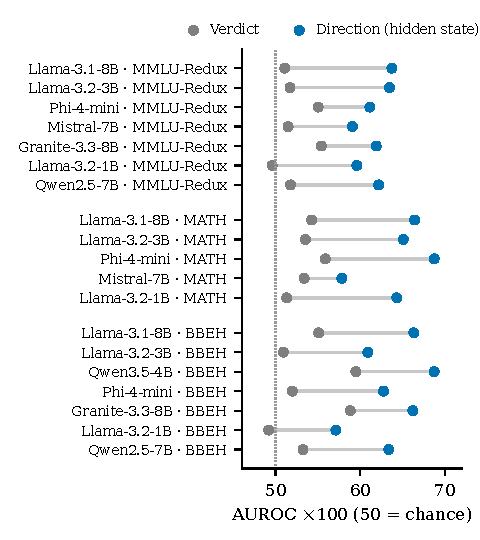
\includegraphics[width=\columnwidth]{fig_gap.pdf}
\caption{Exploratory survey (layer chosen on the evaluated answers): ranking of right above wrong answers to the same question by the verdict and by the correctness direction, for the \R{pool.npairs} judge--benchmark pairs with a gap above 5 points. Not shown (gap $\le 5$): Qwen3.5-9B on all benchmarks, Qwen3.5-4B on MMLU-Redux and MATH, Granite-3.3-8B and Qwen2.5-7B on MATH, Mistral-7B on BBEH.}
\label{fig:gap}
\end{figure}

In an exploratory survey of all \R{pairs.all} judge--benchmark pairs, with the direction learned on one half of the questions and its layer chosen on the other, the verdicts of small judges rank answers barely above chance (\R{pool.verdict.rank} on average over the pairs in Figure~\ref{fig:gap}), and in \R{pool.npairs} pairs the direction ranks \R{gap.lo}--\R{gap.hi} points higher. The gap is absent mostly for the Qwen3.5 judges, whose verdicts already rank within 5 points of their directions. Because the layer is chosen on the evaluated answers, these gaps are optimistic; the primary evaluation below removes that choice.

\begin{takeaway}
As prior work found for probes, a supervised linear direction in small judges' hidden states ranks answers better than their verdicts. This gap is our starting point, not our finding.
\end{takeaway}

\subsection{Closing the Gap}
\label{sec:close}

\begin{table*}[t]
\centering
\small
\begin{tabular}{l c rr rr rr rr}
\toprule
& Verdict & \multicolumn{2}{c}{Reason first} & \multicolumn{2}{c}{Stretch $\times$11} & \multicolumn{2}{c}{Direction} & \multicolumn{2}{c}{Verdict + dir.} \\
\cmidrule(lr){3-4}\cmidrule(lr){5-6}\cmidrule(lr){7-8}\cmidrule(l){9-10}
& Rank / BoN & Rank & BoN & Rank & BoN & Rank & BoN & Rank & BoN \\
\midrule
All questions & 53.3 / 61.6 & $-$0.9 & $-$1.8 & \textbf{+4.3} & \textbf{+4.2} & \textbf{+9.8} & \textbf{+8.9} & \textbf{+6.5} & \textbf{+6.4} \\
Judge cannot solve & 50.8 / 58.3 & $-$0.2 & $-$1.1 & \textbf{+4.2} & \textbf{+4.2} & \textbf{+10.1} & \textbf{+9.6} & \textbf{+6.5} & \textbf{+6.6} \\
\bottomrule
\end{tabular}

\caption{Gains over the verdict on the full answer pools (equal-weight means over judge--benchmark pairs; bold: 95\% interval above 0). Top: the primary evaluation, every choice made on training questions and evaluated on held-out questions; the stretch column is the rule (stretch if the inner gap exceeds 5 points, else the verdict); reasoning first is on the \R{psc.n} of these pairs with a reasoning run. Bottom: the exploratory \R{pool.npairs} pairs with an in-sample gap above 5 points, layer and stretch layer chosen on the evaluated answers (descriptive). Rank: ranking ($\times$100). BoN: best-of-$n$ accuracy, the share of questions with a right and a wrong answer where the top-scored answer is right. $^\ddagger$Questions the judge answered wrong on its one sampled attempt (held out: \R{outer.npairs.unsolved} pairs with such labels).}
\label{tab:readout}
\end{table*}

\paragraph{Reading the direction closes most of the gap; stretching closes part of it.} Held out (Table~\ref{tab:readout}, top), the direction ranks \R{outer.direct.gain.ci} points above the verdict and picks the right answer \R{outer.direct.bon} points more often in best-of-$n$ selection; verdict + direction gains \R{outer.sum.gain.ci}. The rule, which edits the judge's forward pass and so changes its own verdict, gains \R{outer.rule.gain.ci}, \R{outer.recovered.ci} of the direction's gain; a random direction stretched at the same layer changes nothing (\R{outer.random.gain.ci}). The rule fails for one pair: Qwen2.5-7B on MATH passes the inner gap check in both folds and stretching lowers its ranking (\R{outer.qwen2.5-7b.math.rule}; Appendix~\ref{app:outer}). Over \R{ps.splits.n} further random splits of the questions, the direction's pooled gain ranges from \R{ps.splits.lo} to \R{ps.splits.hi}. This is a nested re-analysis of answers we had already studied, not a prospective test on untouched data. On the exploratory selected pairs, choosing layers on the evaluated answers gives larger gains (Table~\ref{tab:readout}, bottom; Appendix~\ref{app:explore}).

\paragraph{Brief reasoning does not help.} On the \R{psc.n} primary pairs with a reasoning run, letting the judge reason before its verdict changes ranking by \R{psc.cot.gain.all.ci}. Prompted to reason briefly, the judges write short justifications (median \R{cot.tok.median} tokens), and for some almost none (Appendix~\ref{app:prompts}); we do not test longer, solve-first reasoning.

\paragraph{When is stretching worth it?} Reading the direction costs nothing beyond the verdict's forward pass (a dot product with a stored state at one layer); stretching re-reads the last token with an edited state, about one extra token step. The direction ranks better than the rule on every measure we use, including best-of-$n$ (\R{outer.direct.bon} against \R{outer.rule.bon}) and a fixed review budget: flagging the 10\% of answers with the lowest scores catches \R{psr.verdict.10.caught}\% of wrong answers with the verdict, \R{psr.direct.10.caught}\% with the direction (\R{psr.direct.10.caught_gain.ci}) and \R{psr.rule.10.caught}\% with the rule (\R{psr.rule.10.caught_gain.ci}; 20\% and 30\% budgets in Appendix~\ref{app:explain}), as \citet{gulati2026auditing} found for probes on MATH. Stretching is useful only where a pipeline must consume the judge's own verdict, for example its accept rate or generated text, rather than an external score; it needs the same labels and hidden-state access as the readout.

\begin{takeaway}
With every choice made on training questions and evaluated on held-out questions, reading a supervised correctness direction gains about 8 points of ranking over a small judge's verdict, and stretching it at one layer recovers \R{outer.recovered.ci} of that gain in the judge's own verdict. Brief reasoning before the verdict, as prompted here, does not help.
\end{takeaway}

\subsection{What the Gain Consists Of}
\label{sec:what}

The answering models differ in accuracy and in how they write, so a score that tells them apart can rank answers well without checking them. On the primary pairs, with the same folds and layers, we test how much of the gain this pattern accounts for (details in Appendix~\ref{app:explain}).

\paragraph{The gain is concentrated in different-model pairs.} On MMLU-Redux and MATH (the \R{ps.npairs.mm} primary pairs where several answers come from one model) we split each pool's right-vs-wrong pairs by whether the two answers were written by the same model. The direction gains \R{psm.direct.gain.diff.ci} over the verdict on different-model pairs and \R{psm.direct.gain.same.ci} on same-model pairs; the paired difference is \R{psm.direct.diff_minus_same.ci}. The rule shows the same pattern (\R{psm.rule.gain.diff.ci} against \R{psm.rule.gain.same.ci}; difference \R{psm.rule.diff_minus_same.ci}). The same-model intervals do not exclude gains of a few points. Different-model pairs may also be easier to check, for example if a weaker model's wrong answers are more obviously wrong, so this split alone does not show that the different-model gain lacks checking value.

\paragraph{Surface features: no detected difference on average, opposite signs by benchmark.} A linear model of nine features of the answer text (length, line count, bold and \LaTeX{} markup, step headers, hedging, confident and self-correcting words, a final-answer line), fitted on training questions, ranks right above wrong at \R{ps.surface.level.all.ci}, against \R{ps.direct.level.all.ci} for the direction and \R{ps.verdict.level.all.ci} for the verdict. On identical answers the surface model minus the direction is \R{ps.surface_minus_direct.all.ci}: no difference is detected, which does not make them equivalent. The average hides opposite signs: the surface model ranks above the direction on MMLU-Redux (\R{psb.mmlu.surface_minus_direct.all.ci}) and MATH (\R{psb.math.surface_minus_direct.all.ci}) but well below it on BBEH (\R{psb.bbeh.surface_minus_direct.all.ci}), where it does not beat the verdict (\R{psb.bbeh.surface.gain.all.ci}). The MMLU-Redux and MATH pools make such cues informative: on MATH, \R{fmt.math.nemo.0.bare}\% of Nemotron's wrong answers but \R{fmt.math.nemo.1.bare}\% of its right ones are a bare final line (``The answer is: 84''). These features are not necessarily irrelevant style: a bare final line, or a long answer full of self-corrections, can reflect a real failure of reasoning.

\paragraph{The direction adds to the features, and they make different errors.} Linear residualization of the direction on the features, with the residualizer fitted to inner cross-fitted training scores, reduces its ranking gain over the verdict by \R{ps.resid_inner_removed.all.ci} under this procedure: about two thirds of the gain survives (\R{psb.mmlu.resid_inner_kept.all} on MMLU-Redux, \R{psb.math.resid_inner_kept.all} on MATH, \R{psb.bbeh.resid_inner_kept.all} on BBEH). AUROC is not additive, so this percentage is not a share of the direction's information. A complementary test fits pairwise logistic models on training pairs: adding the direction to the features raises held-out ranking by \R{ps.pw_sd_minus_s.all.ci} and lowers held-out log loss per pair from \R{ps.ll.surface} to \R{ps.ll.surfacedirect} (\R{ps.ll.sd_minus_s.ci}); adding the features to the direction raises ranking by \R{ps.pw_sd_minus_d.all.ci}. On same-model pairs the direction adds nothing detectable to the features (\R{ps.pw_sd_minus_s.same.ci}). The two scores also err on different pairs: of the test pairs, \R{pso.surface.direct.all.both}\% are ranked correctly by both, \R{pso.surface.direct.all.aonly}\% only by the surface model and \R{pso.surface.direct.all.bonly}\% only by the direction. Residualization, like the subspace removal below, measures overlapping predictive information, not that formatting causes the judge's signal.

\paragraph{On MMLU-Redux, directions that separate answering models carry most of the gain.} Within each question and correctness class we take the paired difference between the states of two models' answers (Qwen3.6-35B vs Qwen3.5-4B, Nemotron vs Qwen3.5-4B), fitted on training questions (Appendix~\ref{app:auth}). Projecting these two \emph{authorship directions} out of the correctness direction removes \R{psb.mmlu.c_perp_removed.all.ci} of its gain over the verdict on MMLU-Redux but only \R{psb.math.c_perp_removed.all.ci} on MATH. On the exploratory selected pairs, 2-D subspaces fitted after shuffling the answering-model labels, and random 2-D subspaces, remove far less (Appendix~\ref{app:auth}). Removing a subspace shows that the readout relies on it; it does not show that authorship as such causes the gain.

\paragraph{A controlled edit: the verdict checks, the direction does not add.} To change correctness with the answering model, wording and format held fixed, we took one right Qwen3.5-4B answer to each of \R{edit.problems} MATH problems and had Kimi-K3.1-Pro, from a family that is neither a judge nor Qwen, change one intermediate step to a wrong value and carry it consistently to a different final answer, leaving all other text unchanged. The protocol was fixed before scoring (Appendix~\ref{app:edit}). Automatic filters (GLM-5.3-Flash confirms the new final answer is wrong; identical line counts, markup and wording features; length within 5\%) keep \R{edit.n} pairs, with median character similarity \R{edit.sim}. The four primary judges score both versions with the frozen readouts of the fold in which the problem is held out. The share of pairs in which the original scores above the edit (50 = chance) is \R{edit.verdict.level.ci} for the verdict, \R{edit.direct.level.ci} for the direction (\R{edit.direct.gain.ci} against the verdict), \R{edit.rule.level.ci} for the rule (\R{edit.rule.gain.ci}) and \R{edit.surface.level.ci} for the surface model, chance as intended. Every judge's direction ranks below its verdict. When correctness changes in one checkable step and little else, the verdicts detect the error and the direction adds nothing, so its gain on the main pools does not come from better checking of such errors. These edits are visible single-step mistakes, often an arithmetic slip, which may be easier to check than natural errors, and the direction, fitted on natural answers, must transfer to a new kind of error. Model readers (not people) found no edit that left the answer right and \R{editr.count.cue} with a visible cue; without those, the result is unchanged (\R{editr.direct.gain.ci}).

\begin{takeaway}
On the primary pairs the direction's gain is concentrated in pairs of answers by different models. A linear model of surface features is not detectably different on average (better on MMLU-Redux and MATH, worse on BBEH), linear residualization reduces the gain by about a third, and features and direction make partly different errors. When one step of a same-model solution is edited to be wrong and nothing else changes, the verdicts detect it and the direction does worse. Gains of readouts on mixed answer pools can overstate how much more a judge can check.
\end{takeaway}

\subsection{Checking Answers to Questions the Judge Failed}
\label{sec:beyond}

\begin{table*}[t]
\centering
\small
\begin{tabular}{llr r rrrr}
\toprule
& & & & \multicolumn{4}{c}{Gain over the verdict} \\ \cmidrule(l){5-8}
Benchmark & Answers by & Judges & Verdict & Reason & Stretch & Direction & Verdict \\
& & & & first & $\times$11 & & + dir. \\
\midrule
MATH & Qwen3.5-4B & 5 & 58.3 & $-$1.7 & \textbf{+1.4} & \textbf{+2.6} & \textbf{+2.6} \\
MATH & OLMo-2-7B & 5 & 59.9 & $-$0.8 & $-$1.0 & $-$2.3 & $-$0.7 \\
BBEH & 4 pool models & 6 & 53.6 & $-$0.5 & +0.8 & \textbf{+3.1} & \textbf{+2.1} \\
MMLU-Redux & Qwen3.5-4B & 4 & 46.5 & +1.5 & +0.2 & \textbf{+2.2} & +0.7 \\
MMLU-Redux & OLMo-2-7B & 4 & 50.8 & \textbf{+2.1} & +0.5 & +1.0 & +0.9 \\
\midrule
MATH, failed 9/9$^\dagger$ & Qwen3.5-4B & 1 & 56.8 & $-$0.3 & \textbf{+5.0} & +3.1 & \textbf{+4.7} \\
\bottomrule
\end{tabular}

\caption{Same-model pairs on questions the judge failed on a sampled attempt: verdict ranking (mean over judges; 50 = chance) and mean gains of each readout over the verdict (bold: 95\% interval above 0). Directions and layers are those of the exploratory selected pairs, learned on the main pool. BBEH pairs come from four answering models that are also in the main pool. $^\dagger$Llama-3.1-8B on the \R{strict.nq} MATH questions it failed in all 9 of its own attempts. Per judge: Appendix Table~\ref{tab:smpairs}.}
\label{tab:sm}
\end{table*}

Judges agree with experts mainly on questions they can solve \citep{krumdick2026nofreelabels,tan2025judgebench}. The same-model, failed-question sets remove the answering model as a cue and restrict each judge to questions it answered wrong on a sampled attempt (Table~\ref{tab:sm}, Figure~\ref{fig:sm}). They use the directions of the exploratory selected pairs, learned on the main pool.

\paragraph{Verdicts are above chance on MATH and BBEH, not on MMLU-Redux.} On MATH the verdicts rank same-model pairs at \R{sm.math.qwen.verdict.rank} on average for Qwen3.5-4B's answers (significantly above chance for \R{chance.math.qwen.above} of \R{chance.math.qwen.n} judges) and \R{sm.math.olmo.verdict.rank} for OLMo-2's (\R{chance.math.olmo.above} of \R{chance.math.olmo.n}), and at \R{sm.bbeh.qwen.verdict.rank} on BBEH (\R{chance.bbeh.qwen.above} of \R{chance.bbeh.qwen.n}). On MMLU-Redux no judge is above chance (\R{sm.mmlu.qwen.verdict.rank} and \R{sm.mmlu.olmo.verdict.rank} on average; \R{chance.mmlu.qwen.below} of \R{chance.mmlu.qwen.n} judges are significantly below chance on Qwen3.5-4B's answers). Llama-3.1-8B ranks same-model pairs at \R{strict.verdict.rank} on the \R{strict.nq} MATH problems it failed in all nine of its own attempts. This is consistent with verification being easier than generation for worked solutions \citep{cobbe2021training,song2025mind}, but not for recall questions, where a worked answer offers little to check without the fact; the contrast is between benchmarks, so format and domain are confounded.

\paragraph{For Qwen's MATH answers, part of the verdict's ranking is surface.} The surface model, fitted on each same-model set, ranks Qwen3.5-4B's MATH answers at \R{surf.sm.math.qwen.surface.ci}, above the verdicts, and removing the features from the verdict score lowers its ranking from \R{surf.sm.math.qwen.verdict} to \R{surf.sm.math.qwen.verdict_resid.ci}. For OLMo-2's MATH answers (\R{surf.sm.math.olmo.verdict} to \R{surf.sm.math.olmo.verdict_resid.ci}) and on BBEH (\R{surf.sm.bbeh.qwen.verdict} to \R{surf.sm.bbeh.qwen.verdict_resid.ci}) the verdict's ranking does not rest on these features.

\paragraph{No readout helps consistently.} For Qwen3.5-4B, whose answers are in the pool the direction is learned from, the direction changes MATH ranking by \R{sm.math.qwen.direct.rank.ci}. For OLMo-2, which the direction has never seen, it lowers MATH ranking (\R{sm.math.olmo.direct.rank.ci}), in line with the poor transfer of correctness probes \citep{orgad2025llms,gulati2026auditing}. Stretching changes ranking by \R{sm.math.qwen.x11.rank.ci} for Qwen's MATH answers and \R{sm.math.olmo.x11.rank.ci} for OLMo-2's. Brief reasoning changes MATH ranking by \R{sm.math.qwen.cot.rank.ci} for Qwen's answers and \R{sm.math.olmo.cot.rank.ci} for OLMo-2's, and MMLU-Redux ranking by \R{sm.mmlu.qwen.cot.rank.ci} and \R{sm.mmlu.olmo.cot.rank.ci}, where the verdicts are not above chance.

\begin{figure}[t]
\centering
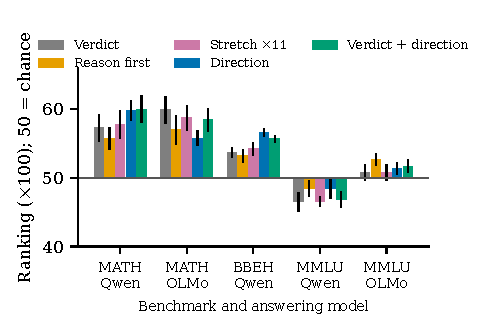
\includegraphics[width=\columnwidth]{fig_sm.pdf}
\caption{Same-model pairs on questions the judge failed on a sampled attempt: ranking by each readout (equal-weight mean over judges; bars: 95\% intervals from the synchronised question bootstrap, which reflect question sampling, not variation between judges). BBEH: four answering models.}
\label{fig:sm}
\end{figure}

\begin{takeaway}
With the answering model fixed and each judge restricted to questions it failed on a sampled attempt, most small judges' verdicts are above chance on MATH and BBEH, and none on MMLU-Redux. For OLMo-2's MATH answers and on BBEH this ranking does not rest on surface features; for Qwen3.5-4B's MATH answers about half of it does. No readout improves on the verdict consistently: the direction's gain for Qwen3.5-4B's answers turns into a loss for OLMo-2's, an answering model it was not learned from.
\end{takeaway}

\subsection{A Larger Judge}
\label{sec:scale}

\begin{table*}[t]
\centering
\small
\begin{tabular}{l rrr rrr rrr rr}
\toprule
& \multicolumn{3}{c}{MMLU-Redux} & \multicolumn{3}{c}{MATH} & \multicolumn{3}{c}{BBEH} & \multicolumn{2}{c}{Same model} \\
\cmidrule(lr){2-4}\cmidrule(lr){5-7}\cmidrule(lr){8-10}\cmidrule(l){11-12}
Judge & Solves & Verdict & Gap & Solves & Verdict & Gap & Solves & Verdict & Gap & MATH & MMLU \\
\midrule
Llama-3.2-1B & 26 & 49.6 & +12.1 & 3 & 51.3 & +12.8 & 5 & 49.2 & +7.9 & 56.2 & 50.0 \\
Llama-3.2-3B & 35 & 51.7 & +11.6 & 10 & 53.5 & +11.8 & 7 & 50.9 & +10.3 & 62.7 & -- \\
Llama-3.1-8B & 44 & 51.1 & +12.6 & 14 & 54.3 & +13.0 & 10 & 55.1 & +11.2 & 58.3 & 47.5 \\
Llama-3.1-70B & 66 & 65.0 & +1.7 & 30 & 61.8 & +4.4 & 15 & 58.6 & +6.0 & 62.9 & 49.4 \\
\bottomrule
\end{tabular}

\caption{Llama judges by size, main answer pools (exploratory protocol). Solves: share of the pool's questions the judge answers correctly (\%). Verdict: the verdict's ranking. Gap: best layer's direction ranking minus the verdict's. Same model: the verdict's ranking on same-model pairs (Qwen3.5-4B answers) on questions the judge failed; Llama-3.2-3B has no MMLU-Redux same-model run.}
\label{tab:scale}
\end{table*}

We ran Llama-3.1-70B through the exploratory pipeline (Table~\ref{tab:scale}). It solves \R{scale.70b.mmlu.solved}\% of MMLU-Redux and \R{scale.70b.math.solved}\% of MATH questions (Llama-3.1-8B: \R{scale.8b.mmlu.solved}\% and \R{scale.8b.math.solved}\%), its verdict ranks at \R{scale.70b.mmlu.says}, \R{scale.70b.math.says} and \R{scale.70b.bbeh.says}, and its direction adds \R{scale.70b.mmlu.gap}, \R{scale.70b.math.gap} and \R{scale.70b.bbeh.gap}, against \R{scale.3b.mmlu.gap} to \R{scale.8b.math.gap} for the smaller Llamas on MMLU-Redux and MATH.

Each judge's failed-question set is different, so we compare sizes on the \R{match.math.nq} MATH questions that all four Llamas failed and that have the same Qwen3.5-4B answers for all of them. There the verdicts rank same-model pairs at \R{match.math.70b} (70B), \R{match.math.3b} (3B), \R{match.math.8b} (8B) and \R{match.math.1b} (1B): the 70B judge is above 8B by \R{match.math.d8b} and above 1B by \R{match.math.d1b}, but not detectably different from 3B (\R{match.math.d3b}), which does not establish that they are equal. On the \R{match.mmlu.nq} shared MMLU-Redux questions all three available sizes are near chance (\R{match.mmlu.70b}, \R{match.mmlu.8b}, \R{match.mmlu.1b}). On the 70B judge's own same-model sets the direction neither helps nor hurts detectably (\R{big.math.sm.qwen.direct.rank.ci} and \R{big.math.sm.olmo.direct.rank.ci} on MATH).

\begin{takeaway}
A 70B judge has a smaller gap (2--6 points), so there is less to close. On the same answers to the same failed MATH questions its verdict ranks above Llama-3.1-8B's and Llama-3.2-1B's but not detectably above Llama-3.2-3B's; on MMLU-Redux all sizes are near chance.
\end{takeaway}

\section{Conclusion}

The supervised readout--verdict gap of small LLM judges can be read out, or partly amplified into the judge's own verdict, and the gain survives when every choice is made on training questions and evaluated on held-out questions. On the same primary pairs, the gain is concentrated in pairs of answers by different models; a linear model of the answers' surface features is not detectably different on average, with opposite signs across benchmarks, and linear residualization on these features leaves about two thirds of the direction's gain, while the two scores make partly different errors. When one step of a same-model solution is edited to be wrong and the rest is held fixed, the verdict detects the error and the direction adds nothing.
On same-model answers to questions the judge failed, what remains is a modest ability to check worked solutions that the verdict already has and that no readout consistently extends. Evaluations of judges and of probes on judges should fix their analysis population in advance and report rankings on same-model pairs and on questions the judge failed, a surface-feature baseline, and an answering model held out from any fitting.

\section*{Limitations}

We study judges with thinking disabled, brief reasoning only, and one larger judge. The primary evaluation covers four judges (\R{outer.npairs} of the \R{pairs.all} judge--benchmark pairs) and re-analyses data we had already studied; it is not a prospective test on untouched questions, and its intervals do not cover refitting the directions or other model families. The same-model and scale analyses use the directions and layers of the exploratory selected pairs. The answer pools come from three models on MMLU-Redux and MATH, whose formats differ by model and correctness; other pools could carry fewer such cues. The same-model sets use questions selected by one judge and two answering models; the OLMo-2 MATH set is small (742 answers to 154 questions), BBEH's answering models all appear in the direction's training pool, and Qwen3.5-4B grades its own answers in the Qwen sets. Failed-question labels come from one sampled answer of the judge, except in the nine-attempt MATH set, and do not show that a judge cannot solve a question. Several judges write almost no reasoning under our brief-reasoning prompt, so our reasoning results do not speak to longer, solve-first reasoning. Our surface features are a fixed, hand-chosen set, and residualization and subspace removal are linear. The controlled-edit test covers one benchmark, one answering model and one editing model, with visible single-step errors checked by automatic filters and model readers, not by people.
The direction needs labelled answers and hidden-state access, and ranking ignores the decision threshold that stretching shifts.

\section*{Ethical Considerations}

We study open models on public benchmarks. Readout gains measured on answers from models of different strength can overstate a judge's reliability; we recommend same-model controls.

\bibliography{refs}

\appendix
\section{Answer Pools}
\label{app:data}

\begin{table}[h]
\centering
\small
\begin{tabular}{llrr}
\toprule
Benchmark & Answering model & Answers & Right \\
\midrule
MMLU-Redux & Qwen3.5-4B & 1,652 & 43\% \\
 & Qwen3.6-35B-A3B & 922 & 81\% \\
 & Nemotron-3-Super-120B & 922 & 72\% \\
\midrule
MATH & Qwen3.5-4B & 1,194 & 50\% \\
 & Qwen3.6-35B-A3B & 602 & 86\% \\
 & Nemotron-3-Super-120B & 588 & 75\% \\
\midrule
BBEH & 8 models & 2,244 & 34--58\% \\
\bottomrule
\end{tabular}
\caption{Main answer pools. BBEH answers come from Qwen3.5-4B, Qwen3.5-9B, Qwen3.6-35B-A3B, Nemotron-3-Nano-30B, Nemotron-3-Super-120B, DeepSeek-V3.1, gpt-oss-20b and gpt-oss-120b. All answers end with a final answer line; MMLU-Redux answers are graded by their final letter against the expert key, MATH answers by GLM-5.3-Flash against the reference (exact matches skip the grader), BBEH answers by the benchmark's matching rule.}
\label{tab:data}
\end{table}

\section{Judge Prompts}
\label{app:prompts}

All judges see one user turn. For MMLU-Redux (MATH and BBEH differ only in the first line: ``a math problem'', ``a reasoning question'', with \texttt{[PROBLEM]} for MATH):

\begin{quote}\small\ttfamily
You are grading an AI assistant's answer to a multiple-choice question.\\[2pt]
[QUESTION]\\ \{question\}\\[2pt]
[ASSISTANT'S ANSWER]\\ \{answer\}\\[2pt]
Is the assistant's final answer correct? Only the final answer matters, not the style of the reasoning. Reason briefly, then end with exactly one line: "VERDICT: CORRECT" or "VERDICT: INCORRECT".
\end{quote}

For the forced verdict and all hidden-state measurements, the assistant turn starts with \texttt{VERDICT:} and we read the next token. For the reasoning baseline, the judge generates freely (greedy, stopping at \texttt{VERDICT:}; at most 8,192 tokens in a 32K window for BBEH and for Llama-3.1-8B on MATH, 1,536 tokens in a 16K window otherwise) and we read the next token after appending \texttt{VERDICT:} to its reasoning. Runs that never write a verdict within the budget (mostly Qwen3.5-4B and Llama-3.1-8B on BBEH, 2--8\% of their answers) are repetitive loops; they are scored the same way. The verdict score uses the first tokens of `` CORRECT'' and `` INCORRECT''.

\section{Layer Rule and Fresh Test}
\label{app:rule}

\paragraph{Rule, fixed before the main run.} Gap check: stop if the gap is $\le 5$. Push test: on 400 random answers, the accept rate at $-8$ and $+8$ standard deviations along the direction at every second layer; a layer responds if the accept rate rises by at least 10 points. Layer: the best-ranking responding layer; if none responds, the best-ranking layer. Stretch: $\times$11 at that layer only, along the direction and along a random direction; $\times$4 and $\times$21 are recorded as secondary readouts.

\paragraph{Revision after a failure.} Mistral-7B on MMLU-Redux accepts 99\% of answers, so no push changes its decision, although the verdict score follows the direction (within-question correlation $+0.54$ to $+0.85$ from layer 18). We therefore measure the response on the verdict score: sensitivity is the mean change in verdict score per standard deviation pushed, divided by the verdict score's within-question standard deviation, and a layer responds if its sensitivity is at least 0.05. In a full sweep this picks layer 16 for Mistral-7B on MMLU-Redux ($+2.3$ [$+0.5$, $+3.7$]). The seven original judges were stretched at the layer the original rule chose (for Mistral-7B on MMLU-Redux, layer 4: $-0.7$), and all pooled numbers use those layers; the revised rule chose the layers for Llama-3.2-1B, Qwen2.5-7B and Llama-3.1-70B. In the main text and Table~\ref{tab:pairs}, a pair counts as responding if the verdict's sensitivity at the stretched layer is at least 0.05.

\paragraph{Fresh test.} Before running Llama-3.2-1B and Qwen2.5-7B, new to the study, we wrote down the revised rule and the prediction that every pair with a gap and a responding layer gains with $\times$11 (interval above 0) and that the random direction stays within $\pm1$. It held for Llama-3.2-1B on MMLU-Redux ($+5.4$) and MATH ($+7.9$), and the random direction stayed within $\pm1$ throughout. It failed on BBEH for both judges ($-1.5$ and $+1.0$). In both, the direction's ranking is flat across the responding layers to within split noise, and the rule took the layer where the verdict only begins to respond; a neighbouring layer with a stronger response gains $+6.4$ [$+3.3$, $+10.3$] (Llama-3.2-1B, layer 14) and $+4.6$ [$+1.2$, $+8.2$] (Qwen2.5-7B, layer 22). Qwen2.5-7B on MMLU-Redux has no responding layer; stretching its best-ranking layer still gains $+2.5$ [$+1.1$, $+4.0$].

\paragraph{Strength.} Judges whose verdict responds strongly (sensitivity $\ge 0.2$) do best at $\times$4--$\times$11; weakly responding ones (sensitivity $< 0.08$, mostly BBEH) at $\times$11--$\times$21. $\times$11 is within about two points of the best tested strength for most pairs.

\section{Every Judge and Benchmark}
\label{app:pairs}

\begin{table*}[h]
\centering
\small
\begin{tabular}{ll rr rr rrrr}
\toprule
Bench & Judge & Gap & Gap, 20 splits & Layer & Sens. & Verdict & Reason & Stretch & Direction \\
\midrule
MMLU-Redux & Llama-3.1-8B & +12.6 & +12.2 $\pm$ 0.8 & 16 & 0.13 & 51.1 & 52.6 & 58.0 & 63.7 \\
MMLU-Redux & Llama-3.2-3B & +11.6 & -- & 12 & 0.06 & 51.7 & 46.5 & 55.8 & 63.4 \\
MMLU-Redux & Qwen3.5-9B & +0.8 & -- & \multicolumn{6}{l}{gap $\le$ 5: not stretched} \\
MMLU-Redux & Qwen3.5-4B & +1.2 & -- & \multicolumn{6}{l}{gap $\le$ 5: not stretched} \\
MMLU-Redux & Phi-4-mini & +7.2 & +7.8 $\pm$ 0.4 & 16 & 0.12 & 55.0 & 52.7 & 58.9 & 61.1 \\
MMLU-Redux & Mistral-7B & +7.6 & +7.9 $\pm$ 0.3 & 4$^*$ & -0.00 & 51.5 & 51.3 & 50.8 & 59.1 \\
MMLU-Redux & Granite-3.3-8B & +6.4 & +5.9 $\pm$ 0.5 & 20 & 0.11 & 55.4 & 51.6 & 57.2 & 61.9 \\
MMLU-Redux & Llama-3.2-1B & +12.1 & +11.7 $\pm$ 0.5 & 10 & 0.05 & 49.6 & 50.9 & 55.0 & 59.6 \\
MMLU-Redux & Qwen2.5-7B & +10.3 & +10.0 $\pm$ 0.7 & 20$^*$ & 0.04 & 51.8 & 50.0 & 54.3 & 62.2 \\
MMLU-Redux & Llama-3.1-70B & +1.7 & +1.4 $\pm$ 0.2 & 34 & 0.27 & 65.0 & 62.6 & 64.9 & 66.8 \\
\midrule
MATH & Llama-3.1-8B & +13.0 & -- & 16 & 0.26 & 54.3 & 53.0 & 62.5 & 66.4 \\
MATH & Llama-3.2-3B & +11.8 & +11.5 $\pm$ 0.4 & 14 & 0.26 & 53.5 & 52.3 & 59.8 & 65.1 \\
MATH & Qwen3.5-9B & +4.9 & -- & \multicolumn{6}{l}{gap $\le$ 5: not stretched} \\
MATH & Qwen3.5-4B & +2.0 & +2.2 $\pm$ 0.3 & \multicolumn{6}{l}{gap $\le$ 5: not stretched} \\
MATH & Phi-4-mini & +12.9 & +12.5 $\pm$ 0.4 & 14 & 0.12 & 55.9 & 56.2 & 62.1 & 68.7 \\
MATH & Mistral-7B & +5.7 & +5.9 $\pm$ 0.7 & 16 & 0.20 & 53.4 & 53.1 & 55.5 & 57.8 \\
MATH & Granite-3.3-8B & +4.4 & +4.5 $\pm$ 0.3 & \multicolumn{6}{l}{gap $\le$ 5: not stretched} \\
MATH & Llama-3.2-1B & +12.8 & +12.1 $\pm$ 1.1 & 14 & 0.15 & 51.3 & 52.5 & 59.1 & 64.3 \\
MATH & Qwen2.5-7B & +5.0 & +5.0 $\pm$ 0.3 & \multicolumn{6}{l}{gap $\le$ 5: not stretched} \\
MATH & Llama-3.1-70B & +4.4 & +4.5 $\pm$ 0.3 & 34 & 0.25 & 61.8 & 62.5 & 62.3 & 66.3 \\
\midrule
BBEH & Llama-3.1-8B & +11.2 & +9.2 $\pm$ 2.3 & 14$^*$ & 0.04 & 55.1 & 50.8 & 61.8 & 66.3 \\
BBEH & Llama-3.2-3B & +10.3 & +8.8 $\pm$ 3.1 & 14$^*$ & 0.03 & 50.9 & 51.4 & 55.6 & 60.9 \\
BBEH & Qwen3.5-9B & -1.5 & -- & \multicolumn{6}{l}{gap $\le$ 5: not stretched} \\
BBEH & Qwen3.5-4B & +9.3 & +8.0 $\pm$ 1.6 & 20 & 0.08 & 59.5 & 63.9 & 64.7 & 68.7 \\
BBEH & Phi-4-mini & +10.8 & +7.2 $\pm$ 4.2 & 20 & 0.07 & 52.0 & 46.9 & 56.0 & 62.7 \\
BBEH & Mistral-7B & +4.5 & +5.0 $\pm$ 0.8 & \multicolumn{6}{l}{gap $\le$ 5: not stretched} \\
BBEH & Granite-3.3-8B & +7.4 & +6.5 $\pm$ 1.6 & 22 & 0.19 & 58.8 & 53.1 & 65.1 & 66.2 \\
BBEH & Llama-3.2-1B & +7.9 & +5.9 $\pm$ 1.5 & 10 & 0.20 & 49.2 & 52.4 & 47.7 & 57.1 \\
BBEH & Qwen2.5-7B & +10.1 & +8.5 $\pm$ 1.2 & 20 & 0.09 & 53.2 & 54.6 & 54.2 & 63.4 \\
BBEH & Llama-3.1-70B & +6.0 & +4.6 $\pm$ 2.4 & 32 & 0.06 & 58.6 & 57.9 & 60.0 & 64.6 \\
\bottomrule
\end{tabular}

\caption{Every judge--benchmark pair. Gap: best layer's direction ranking minus the verdict's, on the split used for the layer rule; 20 splits: mean $\pm$ standard deviation over 20 random half-splits of the questions (at the best layer). Layer: the stretched layer ($^*$: the verdict's sensitivity there is below 0.05). Sens.: the verdict's sensitivity there. Llama-3.1-70B is the scale check of \S\ref{sec:scale}. Last four columns: ranking ($\times$100) of the forced verdict, the verdict after reasoning, the verdict after stretching $\times$11, and the direction, on the main answer pool.}
\label{tab:pairs}
\end{table*}

\begin{table*}[h]
\centering
\small
\begin{tabular}{lll r rrrrrr}
\toprule
Bench & Judge & Answers by & Groups & Verdict & Reason & Str.\,$\times$4 & Str.\,$\times$11 & Direction & Verd.+dir. \\
\midrule
MATH & Llama-3.1-70B & OLMo-2-7B & 89 & 62.6 & 62.8 & 62.6 & 58.9 & 64.4 & 63.3 \\
MATH & Llama-3.1-70B & Qwen3.5-4B & 280 & 62.9 & 63.3 & 63.7 & 63.1 & 64.0 & 64.6 \\
MATH & Llama-3.1-8B & OLMo-2-7B & 154 & 58.9 & 60.5 & 58.6 & 57.9 & 58.9 & 59.0 \\
MATH & Llama-3.1-8B & Qwen3.5-4B & 350 & 58.3 & 57.4 & 62.0 & 62.2 & 60.5 & 61.8 \\
MATH & Llama-3.1-8B & Qwen3.5-4B, failed 9/9 & 255 & 56.8 & 56.5 & 61.6 & 61.8 & 59.9 & 61.6 \\
MATH & Llama-3.2-1B & OLMo-2-7B & 150 & 54.8 & 54.6 & 54.4 & 54.3 & 53.3 & 52.5 \\
MATH & Llama-3.2-1B & Qwen3.5-4B & 340 & 56.2 & 54.4 & 58.3 & 59.9 & 61.8 & 59.9 \\
MATH & Llama-3.2-3B & OLMo-2-7B & 132 & 60.5 & 58.4 & 60.2 & 60.0 & 56.8 & 60.1 \\
MATH & Llama-3.2-3B & Qwen3.5-4B & 327 & 62.7 & 58.8 & 65.3 & 59.4 & 61.3 & 65.3 \\
MATH & Mistral-7B & OLMo-2-7B & 142 & 58.2 & -- & 58.6 & 56.6 & 56.3 & 57.9 \\
MATH & Mistral-7B & Qwen3.5-4B & 340 & 55.8 & -- & 56.4 & 55.2 & 58.2 & 57.8 \\
MATH & Phi-4-mini & OLMo-2-7B & 102 & 67.0 & 61.4 & 66.0 & 64.7 & 53.3 & 62.7 \\
MATH & Phi-4-mini & Qwen3.5-4B & 307 & 58.5 & 57.7 & 60.2 & 56.4 & 61.5 & 59.5 \\
BBEH & Granite-3.3-8B & 4 pool models & 335 & 50.5 & 51.3 & 53.5 & 53.9 & 56.0 & 54.6 \\
BBEH & Llama-3.1-70B & 4 pool models & 311 & 55.2 & 58.0 & 56.1 & 54.7 & 56.1 & 57.8 \\
BBEH & Llama-3.1-8B & 4 pool models & 303 & 54.3 & 50.1 & 54.6 & 55.4 & 55.7 & 56.6 \\
BBEH & Llama-3.2-1B & 4 pool models & 350 & 53.7 & 53.5 & 54.2 & 49.8 & 55.3 & 54.3 \\
BBEH & Llama-3.2-3B & 4 pool models & 341 & 53.2 & 54.1 & 55.5 & 54.5 & 55.6 & 54.9 \\
BBEH & Phi-4-mini & 4 pool models & 343 & 55.7 & 53.8 & 55.9 & 56.6 & 58.7 & 57.3 \\
BBEH & Qwen3.5-4B & 4 pool models & 210 & 54.4 & 56.2 & 54.8 & 55.2 & 57.9 & 56.2 \\
MMLU-Redux & Granite-3.3-8B & OLMo-2-7B & 193 & 47.7 & 50.4 & 48.8 & 48.7 & 50.6 & 49.1 \\
MMLU-Redux & Granite-3.3-8B & Qwen3.5-4B & 271 & 44.9 & 48.6 & 44.3 & 45.1 & 46.3 & 44.9 \\
MMLU-Redux & Llama-3.1-70B & OLMo-2-7B & 129 & 50.6 & 46.2 & 49.4 & 48.7 & 50.5 & 49.9 \\
MMLU-Redux & Llama-3.1-70B & Qwen3.5-4B & 183 & 49.4 & 50.4 & 49.5 & 46.0 & 48.9 & 49.8 \\
MMLU-Redux & Llama-3.1-8B & OLMo-2-7B & 305 & 53.3 & 52.7 & 53.5 & 53.9 & 53.3 & 53.6 \\
MMLU-Redux & Llama-3.1-8B & Qwen3.5-4B & 401 & 47.5 & 50.3 & 47.8 & 47.5 & 51.0 & 47.4 \\
MMLU-Redux & Llama-3.2-1B & OLMo-2-7B & 241 & 51.5 & 54.6 & 51.1 & 49.5 & 49.3 & 51.9 \\
MMLU-Redux & Llama-3.2-1B & Qwen3.5-4B & 318 & 50.0 & 49.8 & 49.9 & 48.1 & 50.5 & 50.0 \\
MMLU-Redux & Phi-4-mini & OLMo-2-7B & 198 & 50.5 & 53.0 & 50.5 & 50.8 & 51.9 & 52.2 \\
MMLU-Redux & Phi-4-mini & Qwen3.5-4B & 269 & 43.6 & 45.0 & 45.2 & 45.3 & 45.8 & 45.2 \\
\bottomrule
\end{tabular}

\caption{Same-model pairs on questions the judge cannot solve, per judge: ranking ($\times$100) by each readout. Groups: questions with at least one right and one wrong answer from the same answering model.}
\label{tab:smpairs}
\end{table*}

\section{Authorship Directions and Controls}
\label{app:auth}

Per judge and benchmark, at the best-ranking layer and with the same two question halves as the correctness direction, we take, within every question and correctness class that holds answers by both models, the difference between the two models' mean states, and average these paired differences: Qwen3.6-35B-A3B vs Qwen3.5-4B (``own pair'') and Nemotron-3-Super-120B vs Qwen3.5-4B. Table~\ref{tab:auth} reports, on held-out questions, how well the first direction separates answers by its own pair and by the other pair (within question and correctness class; 50 = none, below 50 = reversed), its cosine with the correctness direction, and the ranking of right above wrong answers by the verdict, by the correctness direction, and by the correctness direction with both authorship directions projected out ($\perp$). Llama-3.1-8B on MATH and Llama-3.2-3B on MMLU-Redux were run with a different storage layout and are not in this table; the controls below include them. The Verdict column is recomputed on all answers with stored hidden states and can differ by a few tenths from Table~\ref{tab:pairs}, which uses only questions where every readout has a score.

\paragraph{Controls.} All fits use the training half of the questions; numbers in \S\ref{sec:what} are pooled over the \R{ctl.both.n} main-pool pairs on MMLU-Redux and MATH (\R{ctl.mmlu.n} and \R{ctl.math.n}). \emph{Label shuffles}: within every question and correctness class of the training half, the answering-model labels are permuted, the two paired directions are fitted as before, and their span is projected out of the correctness direction; 100 shuffles per judge. The mean removal over shuffles is at most \R{ctl.mmlu.perm.maxmean} points per judge on MMLU-Redux and \R{ctl.math.perm.maxmean} on MATH (it is often negative: removing two high-variance directions can sharpen the ranking). \emph{Random subspaces}: 100 isotropic random 2-D subspaces per judge, drawn without labels, remove at most \R{ctl.mmlu.iso.max} points. \emph{Within-model fit}: the correctness direction is fitted after centring each question's answers separately for each answering model, so only right-vs-wrong contrasts between answers by the same model enter. \emph{Held-out answering model}: the direction is fitted without one model's answers and scored on that model's same-model pairs; only Qwen3.5-4B has several answers per question, so only it can be held out this way (fitted without it: \R{ctl.ho.c_ho.gain.ci} over the verdict; with it: \R{ctl.ho.c_all.gain.ci}). OLMo-2 in \S\ref{sec:beyond} is a fully held-out answering model.

\paragraph{Why not a variance share.} A simpler measure of authorship is the share of a score's within-question variance that lies between answering models (\R{share.direct.lo}--\R{share.direct.hi}\% for the direction, \R{share.verdict.lo}--\R{share.verdict.hi}\% for the verdict). With one or two answers per model and question, a score shuffled within question already gets \R{share.null.lo}--\R{share.null.hi}\%, and the correctness label itself \R{share.gold.lo}--\R{share.gold.hi}\%, so this share says little about authorship. The pair split and the authorship directions of \S\ref{sec:what} replace it.

\begin{table*}[h]
\centering
\small
\begin{tabular}{ll r rr r rrr rr}
\toprule
& & & \multicolumn{2}{c}{Authorship dir.} & & \multicolumn{3}{c}{Ranking, all pairs} & \multicolumn{2}{c}{Same-model pairs} \\
\cmidrule(lr){4-5}\cmidrule(lr){7-9}\cmidrule(l){10-11}
Bench & Judge & Layer & Own pair & Other pair & cos & Verdict & Dir. & Dir.$\perp$ & Dir. & Dir.$\perp$ \\
\midrule
MMLU-Redux & Llama-3.1-8B & 16 & 78.7 & 30.9 & +0.19 & 51.1 & 63.7 & 58.4 & 60.7 & 59.3 \\
MMLU-Redux & Phi-4-mini & 14 & 79.9 & 32.6 & +0.13 & 55.0 & 62.2 & 56.9 & 54.3 & 55.6 \\
MMLU-Redux & Mistral-7B & 4 & 80.8 & 27.4 & $-$0.05 & 51.5 & 59.1 & 52.7 & 51.5 & 49.4 \\
MMLU-Redux & Granite-3.3-8B & 20 & 85.1 & 29.8 & +0.06 & 55.4 & 61.8 & 58.4 & 57.6 & 57.9 \\
MMLU-Redux & Llama-3.2-1B & 4 & 84.3 & 28.5 & +0.14 & 49.6 & 61.8 & 53.5 & 52.8 & 52.8 \\
MMLU-Redux & Qwen2.5-7B & 20 & 77.6 & 31.4 & +0.19 & 51.8 & 62.1 & 57.6 & 57.0 & 57.6 \\
\midrule
MATH & Llama-3.2-3B & 14 & 84.4 & 42.3 & +0.43 & 53.7 & 65.5 & 62.8 & 61.6 & 62.1 \\
MATH & Qwen3.5-4B & 20 & 66.2 & 52.7 & +0.71 & 66.4 & 68.4 & 69.5 & 64.4 & 68.2 \\
MATH & Phi-4-mini & 14 & 71.3 & 45.5 & +0.76 & 56.0 & 68.9 & 67.1 & 65.2 & 63.1 \\
MATH & Mistral-7B & 2 & 73.1 & 91.2 & +0.52 & 53.4 & 59.1 & 60.8 & 48.2 & 59.2 \\
MATH & Granite-3.3-8B & 22 & 77.1 & 44.3 & +0.68 & 62.5 & 66.9 & 62.3 & 59.1 & 58.5 \\
MATH & Llama-3.2-1B & 14 & 81.0 & 35.3 & +0.44 & 51.9 & 64.7 & 62.3 & 58.9 & 58.7 \\
MATH & Qwen2.5-7B & 20 & 69.0 & 43.5 & +0.57 & 58.5 & 63.5 & 64.4 & 60.0 & 60.7 \\
\bottomrule
\end{tabular}

\caption{Authorship directions (held out). Own pair / other pair: AUROC of the Qwen3.6-vs-Qwen3.5-4B direction for Qwen3.6 vs Qwen3.5-4B answers and for Nemotron vs Qwen3.5-4B answers of equal correctness. cos: with the correctness direction. Ranking of right above wrong answers by the verdict, the correctness direction, and the correctness direction with both authorship directions removed ($\perp$), on all and on same-model pairs.}
\label{tab:auth}
\end{table*}

\section{Best-of-$n$ Selection}
\label{app:bon}

\begin{table*}[h]
\centering
\small
\begin{tabular}{lr rr rrrr}
\toprule
Answers & Judges & Random & Verdict & Reason first & Stretch $\times$11 & Direction & Verdict + dir. \\
\midrule
All questions & 19 & 59.7 & 61.6 & $-$1.7 & \textbf{+2.5} & \textbf{+8.1} & \textbf{+5.4} \\
Judge cannot solve & 19 & 58.4 & 58.3 & $-$1.0 & \textbf{+2.4} & \textbf{+9.0} & \textbf{+5.7} \\
Same model, MATH, Qwen3.5-4B & 5 & 56.3 & 63.6 & $-$4.7 & +0.9 & +0.6 & +1.1 \\
Same model, MATH, OLMo-2-7B & 5 & 36.0 & 47.1 & $-$1.5 & $-$1.5 & $-$3.6 & $-$2.8 \\
Same model, BBEH, 4 pool models & 6 & 47.5 & 50.3 & $-$0.9 & \textbf{+1.5} & \textbf{+2.3} & \textbf{+1.9} \\
Same model, MMLU-Redux, Qwen3.5-4B & 4 & 48.2 & 44.4 & +2.1 & $-$1.2 & +0.2 & $-$1.7 \\
Same model, MMLU-Redux, OLMo-2-7B & 4 & 43.2 & 41.7 & +2.3 & $-$0.5 & +1.4 & +0.7 \\
\bottomrule
\end{tabular}

\caption{Best-of-$n$ accuracy: the share of groups (questions; question $\times$ answering model for same-model sets; only groups with at least one right and one wrong answer) in which the top-scored answer is right, for random choice and the forced verdict, and the gain of each readout over the verdict (mean over judges; bold: 95\% interval above 0).}
\label{tab:bon}
\end{table*}

\section{Pooling}
\label{app:pool}

The primary estimate is the equal-weight mean over judge--benchmark pairs, with questions resampled within benchmark (2,000 draws) and the same draws for every judge and readout. An earlier version weighted pairs by the inverse variance of their own intervals and treated judges as independent; that weighting favours pairs with tight intervals, which are often those with small gains, and its intervals are too narrow because judges grade the same answers. On the main pools it gives \R{legacy.pool.direct.rank.ci} for the direction, \R{legacy.pool.sum.rank.ci} for verdict + direction, \R{legacy.pool.x11.rank.ci} for stretching and \R{legacy.pool.cot.rank.ci} for reasoning first, against \R{pool.direct.rank.ci}, \R{pool.sum.rank.ci}, \R{pool.x11.rank.ci} and \R{pool.cot.rank.ci} here. Weighting every question equally (the mean of per-question AUROCs) instead of every right--wrong pair gives \R{pool.direct.rank_macro.ci}, \R{pool.sum.rank_macro.ci}, \R{pool.x11.rank_macro.ci} and \R{pool.cot.rank_macro.ci}. All of these are conditional on the judges and benchmarks studied; they do not generalise to a population of judges.

\section{Surface Features}
\label{app:surface}

Features of the answer text (the block the judge grades): log characters, log lines, count of bold markers, count of \texttt{\$}, count of the word ``step'', counts of hedge words (maybe, might, perhaps, possibly, probably, likely, approximately, I think, I believe, not sure, unclear, assume), confident words (clearly, definitely, certainly, obviously, indeed, undoubtedly, must be) and self-correction words (wait, actually, however, recheck, double-check, let me re-, mistake, correction), and whether the text contains ``the answer is''. Features, labels and scores are centred within question and the features standardised; a least-squares fit on one half of the questions predicts the other half. \emph{Surface}: correctness predicted from the features. \emph{Direction without surface}: the direction score minus its prediction from the features. On same-model pairs the surface model ranks at \R{surf.surface.level.same} (verdict \R{surf.verdict.level.same}, direction \R{surf.direct.level.same}). On MMLU-Redux the cue is length rather than bare lines: \R{fmt.mmlu.nemo.0.bare}\% of Nemotron's wrong and \R{fmt.mmlu.nemo.1.bare}\% of its right answers are bare final lines, but \R{fmt.mmlu.q36.0.long}\% of Qwen3.6's wrong and \R{fmt.mmlu.q36.1.long}\% of its right answers exceed 8,000 characters. In the format-trimmed pools (answers of 100--8,000 characters) the direction gains \R{surf.trim.direct.gain.same} on same-model and \R{surf.trim.direct.gain.diff} on different-model pairs.

\section{Held-Out Evaluation of the Recipe}
\label{app:outer}

The scope was fixed before running: Llama-3.1-8B, Qwen2.5-7B, Phi-4-mini and Granite-3.3-8B on MMLU-Redux, MATH and BBEH, \R{outer.npairs} pairs, including two that the main pool leaves out because their in-sample gap is at most 5 points (\R{outer.notpaper}). The outer folds are the paper's two question halves; each is the test set once. On the training half only: (1)~the direction at every candidate layer (class-mean difference after centring by question); (2)~an inner split of the training questions gives each layer's cross-fitted ranking and the verdict's; the best layer is the readout layer, and the pair is eligible if it beats the verdict by more than 5 points; (3)~the push test ($\pm$8 standard deviations on 400 training answers, no labels) gives each layer's sensitivity, and the stretch layer is the best-ranking layer with sensitivity $\ge 0.05$, or the best-ranking layer if none responds. On the test half: the direction at the readout layer, the verdict stretched ($\times$11) along the training direction at every candidate layer, and a random direction stretched at the chosen layer. The rule takes the stretched verdict if the fold is eligible and the verdict otherwise. \R{outer.folds.eligible} of the \R{outer.folds} folds were eligible (Table~\ref{tab:outer}). Picking the stretch layer after seeing the test results would add \R{outer.optimism.mean} point on average.

\begin{table*}[t]
\centering
\small
\begin{tabular}{ll cc r rrr rr}
\toprule
& & & & & \multicolumn{3}{c}{Held out: gain over verdict} & \multicolumn{2}{c}{Paper (in-sample choice)} \\
\cmidrule(lr){6-8}\cmidrule(l){9-10}
& Judge & Eligible & Layer & Verdict & Direction & Rule & Random & Direction & Stretch \\
\midrule
MMLU-Redux & Llama-3.1-8B & y/y & 16/16 & 51.1 & +12.1 & +7.0 & +0.2 & +12.6 & +6.9 \\
MMLU-Redux & Phi-4-mini & y/y & 14/18 & 55.0 & +7.2 & +3.8 & $-$0.1 & +6.1 & +3.9 \\
MMLU-Redux & Granite-3.3-8B & y/y & 20/20 & 55.4 & +6.5 & +1.7 & +0.1 & +6.5 & +1.7 \\
MMLU-Redux & Qwen2.5-7B & y/y & 20/20 & 51.8 & +10.3 & +2.5 & 0.0 & +10.4 & +2.5 \\
\midrule
MATH & Llama-3.1-8B & y/y & 20/16 & 54.4 & +12.3 & +8.8 & $-$0.4 & +12.2 & +8.2 \\
MATH & Phi-4-mini & y/y & 14/16 & 56.0 & +10.2 & +5.1 & +0.1 & +12.8 & +6.2 \\
MATH & Granite-3.3-8B & n/n & 20/20 & 62.5 & +4.0 & 0.0 & +0.1 & -- & -- \\
MATH & Qwen2.5-7B & y/y & 20/20 & 58.5 & +8.0 & $-$1.4 & $-$0.3 & -- & -- \\
\midrule
BBEH & Llama-3.1-8B & n/y & 18/16 & 55.1 & +7.7 & +3.5 & $-$0.2 & +11.2 & +6.8 \\
BBEH & Phi-4-mini & y/y & 10/20 & 52.0 & +6.4 & +2.7 & +0.4 & +10.8 & +4.0 \\
BBEH & Granite-3.3-8B & n/y & 38/24 & 58.8 & +3.2 & +1.3 & $-$0.8 & +7.4 & +6.3 \\
BBEH & Qwen2.5-7B & n/y & 22/22 & 53.2 & +8.6 & +2.6 & +0.7 & +10.1 & +1.0 \\
\bottomrule
\end{tabular}

\caption{Held-out evaluation of the recipe. Eligible and Layer: whether the inner gap exceeded 5 points, and the chosen stretch layer, in each of the two folds. Verdict: ranking ($\times$100). Held out: gains over the verdict of the direction, the rule (stretch if eligible, else the verdict) and a random direction stretched at the chosen layer. Paper: gains with the layer chosen on the evaluated questions (--: not stretched in the main pool).}
\label{tab:outer}
\end{table*}

\section{Compute}

Hidden-state capture, push tests and stretching ran on single H100 GPUs with Hugging Face Transformers (one forward pass per answer, plus a few edited re-reads of the last token, which can reuse the key-value cache); about one GPU-hour per judge--benchmark pair. Llama-3.1-70B ran on two H200 GPUs on a university cluster (2--3 hours per benchmark for capture, push test and stretching; about 4 hours of vLLM for its own answers and the reasoning baseline). Reasoning judgments and OLMo-2 answers used vLLM. Directions and readouts are computed on CPU from stored hidden states.


\end{document}
